\documentclass{article}
\usepackage{graphicx} % Required for inserting images
\graphicspath{ {./assets/} }
\usepackage{stackengine,scalerel}
\usepackage{enumitem}
\usepackage[utf8]{inputenc}
\usepackage{bm}
\usepackage{babel}
\usepackage{amsmath}
\usepackage{dsfont}
\usepackage{mathtools}% Loads amsmath
\usepackage{amssymb}
\usepackage{multirow}
\usepackage{arydshln}
\usepackage{listings}
\usepackage{stackrel}
\usepackage{setspace}
\usepackage{multicol}
\usepackage{stmaryrd}
\usepackage{hyperref}
\usepackage{indentfirst}
\usepackage[]{caption}
\usepackage{xcolor}
\usepackage{xurl}
\setlength\parindent{0pt}
\allowdisplaybreaks
\usepackage{geometry}
\geometry{verbose,tmargin=1cm,bmargin=2cm,lmargin=2cm,rmargin=2cm}


\usepackage[T1]{fontenc}
\onehalfspacing

\makeatletter
%%%%%%%%%%%%%%%%%%%%%%%%%%%%%% Textclass specific LaTeX commands.
\newenvironment{lyxlist}[1]
    {\begin{list}{}
        {\settowidth{\labelwidth}{#1}
         \setlength{\leftmargin}{\labelwidth}
         \addtolength{\leftmargin}{\labelsep}
         \renewcommand{\makelabel}[1]{##1\hfil}}}
    {\end{list}}

%%%%%%%%%%%%%%%%%%%%%%%%%%%%%% User specified LaTeX commands.

\makeatother

\title{COMP4702 Machine Learning Project}
\author{Hugo Burton}
\date{April 2024}

% Footer
\usepackage{fancyhdr}
\pagestyle{fancy}
\fancyhf{} 
\fancyfoot[L]{COMP4702 Machine Learning Project Report}
\fancyfoot[C]{Hugo Burton}
\fancyfoot[R]{\thepage}
\renewcommand{\headrulewidth}{0pt} % Remove the line at the top of the page
\renewcommand{\footrulewidth}{0.4pt} % Add a line just above the footer

\begin{document}

\maketitle
% Reset page style to fancy (after maketitle)
\thispagestyle{fancy}

% cmds
\newcommand{\PP}{\mathbb{P}}
\newcommand{\cc}{^{\mathsf{c}}}

% Double struck characters
\newcommand{\A}{\ensuremath{\mathbb{A}}}
\newcommand{\C}{\ensuremath{\mathbb{C}}}
\newcommand{\E}{\ensuremath{\mathbb{E}}}
\newcommand{\I}{\ensuremath{\mathbb{I}}}
\newcommand{\J}{\ensuremath{\mathbb{J}}}
\newcommand{\N}{\ensuremath{\mathbb{N}}}
\newcommand{\pr}{\ensuremath{\mathbb{P}}}
\newcommand{\Q}{\ensuremath{\mathbb{Q}}}
\newcommand{\R}{\ensuremath{\mathbb{R}}}
\newcommand{\T}{\ensuremath{\mathbb{T}}}
\newcommand{\X}{\ensuremath{\mathbb{X}}}

\newcommand{\qed}{\hfill\blacksquare}

\newcommand{\scriptG}{\mathcal{G}}
\newcommand{\scriptN}{\mathcal{N}}
\newcommand{\scriptI}{\mathcal{I}}
\newcommand{\scriptL}{\mathcal{L}}
\newcommand{\scriptR}{\mathcal{R}}

\newcommand{\var}{\text{Var}}

\newcommand{\bs}[1]{\boldsymbol{#1}} % remaps \bsboldsymbol to just \bs
\newcommand{\dif}[1]{\text{d#1}}
\newcommand{\ddx}{\frac{\text{d}}{\dif{x}}}

% Custom commands for this document
\newcommand{\ito}{\ensuremath{\text{It}\hat{\text{o}}}}

\noindent
Student Number: s4698512\\
Due: Friday $24^{\text{th}}$ May 2024 @ 2pm

\section{Introduction}

\subsection{Dataset}

This report is an investigation into the quantitative traits of fruit flies, known scientifically as the species \textit{Drosophila aldrichi} and \textit{D. buzzatii}. The data, collected in 1994 captures a range of traits of $n = 1731$ flies located on the East coast of Australia. The attached report on the dataset aims to contribute to understanding the factors driving latitudinal variation in size-related traits in the two species, considering both genetic adaptation and phenotypic plasticity in response to environmental conditions. \\
\\
Fruit flies are a pest to many kinds of agriculture. Adult female flies lay their eggs within fruit and vegetable crops leading to their larvae hatching inside. These larvae then proceed to each the fruit from the inside out, causing rotting and thus destroying the crop. (Department of Agriculture, 2023)

\newpage
\subsection{Preliminary Observations of the Datasets}

Prior to determining an objective for this report, the dataset was analysed from a purely morphological perspective.

\subsubsection{Thorax and Wing Traits Dataset}

A correlation plot of the \texttt{Thorax \& wing traits} dataset is shown below. Evidently the columns species, population, temperature and sex all show a small magnitude of correlation with columns \texttt{Thorax length} through to \texttt{wing loading}. 

Longitude and latitude do show some correlation (other than with each other) - this could be interesting to investigate, though may not produce the best results from a classifier with this data alone. \\
\\
The columns \texttt{Thorax length} through to \texttt{wing loading} show a highly positive correlation as seen in the bottom-right of the matrix, indicating these variables are very tightly related to each other. For example, we could say a fly with a higher than average Thorax length also very likely has a higher then average wing loading. \\
\\
We note some columns as having no correlation with any other columns, namely \texttt{year start} and \texttt{year end}. Looking at the raw data, we see these are constant for all rows. In any analysis it would be a good decision to strip these from the model as they don't provide any additional information for classification purposes. Additionally, it was observed that there exist only distinct \texttt{Latitude} and \texttt{Longitude} which are unique for each population. To make the classification fair, it would also make sense to remove these prior to training.

\begin{figure}[htb]
    \centering
    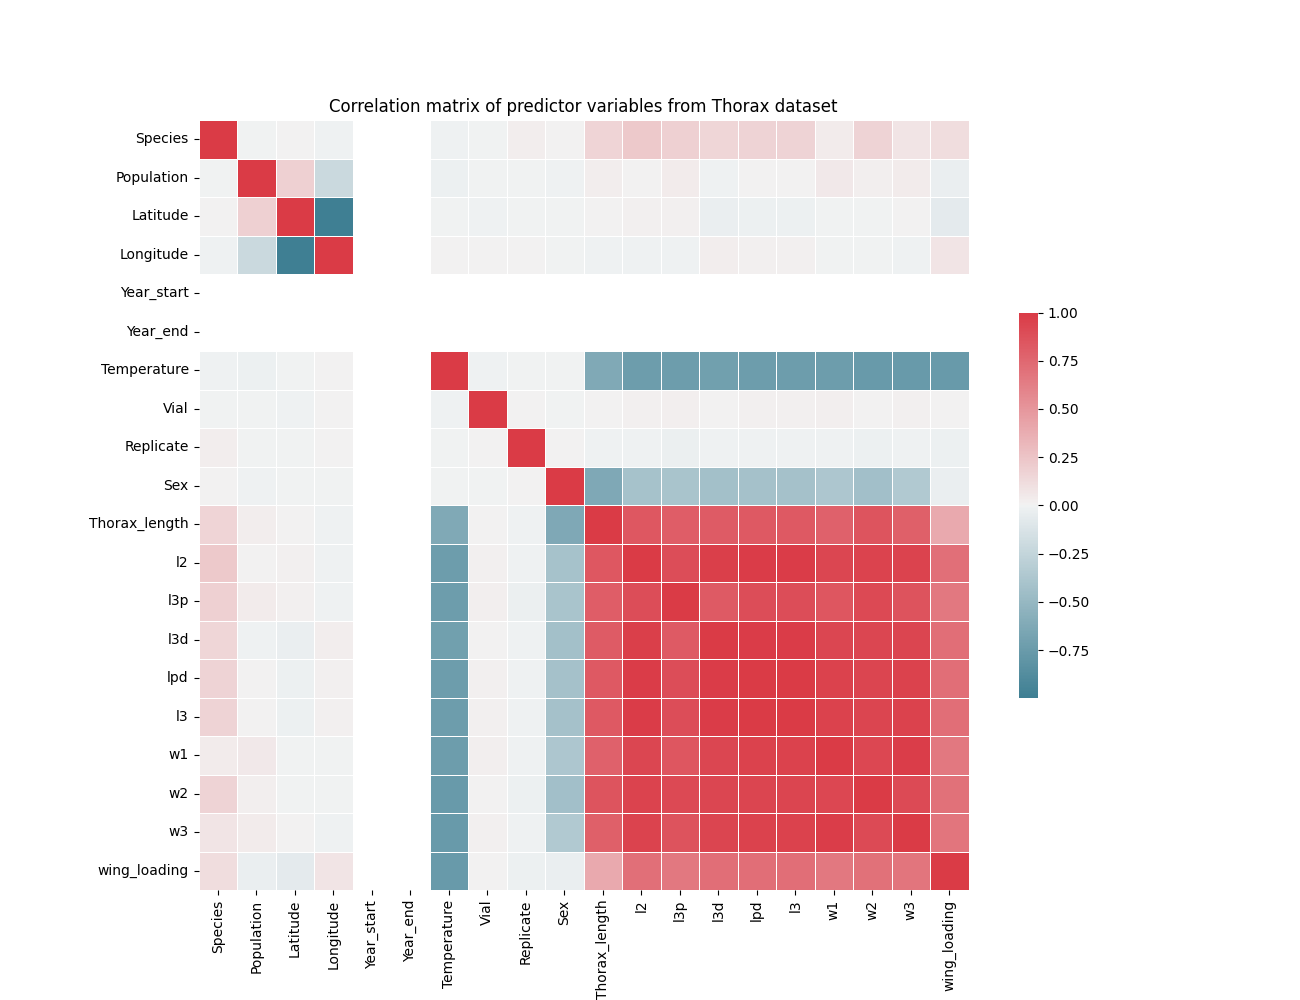
\includegraphics[width=0.8\columnwidth]{plots/Thorax_corr_matrix.png}
    \caption{Thorax and Wing Traits Correlation Matrix}
    \label{fig:thorax_wing_traits_corr_matrix}
\end{figure}

\newpage
The \texttt{Wing Traits and Asymmetry} dataset does show correlation between each of the wing asymmetry traits, however, it shows little to no correlation between wing asymmetry and species and population. Meaning it is potentially not a good candidate dataset for making predictions about the fly's species and population.

\begin{figure}[htb]
    \centering
    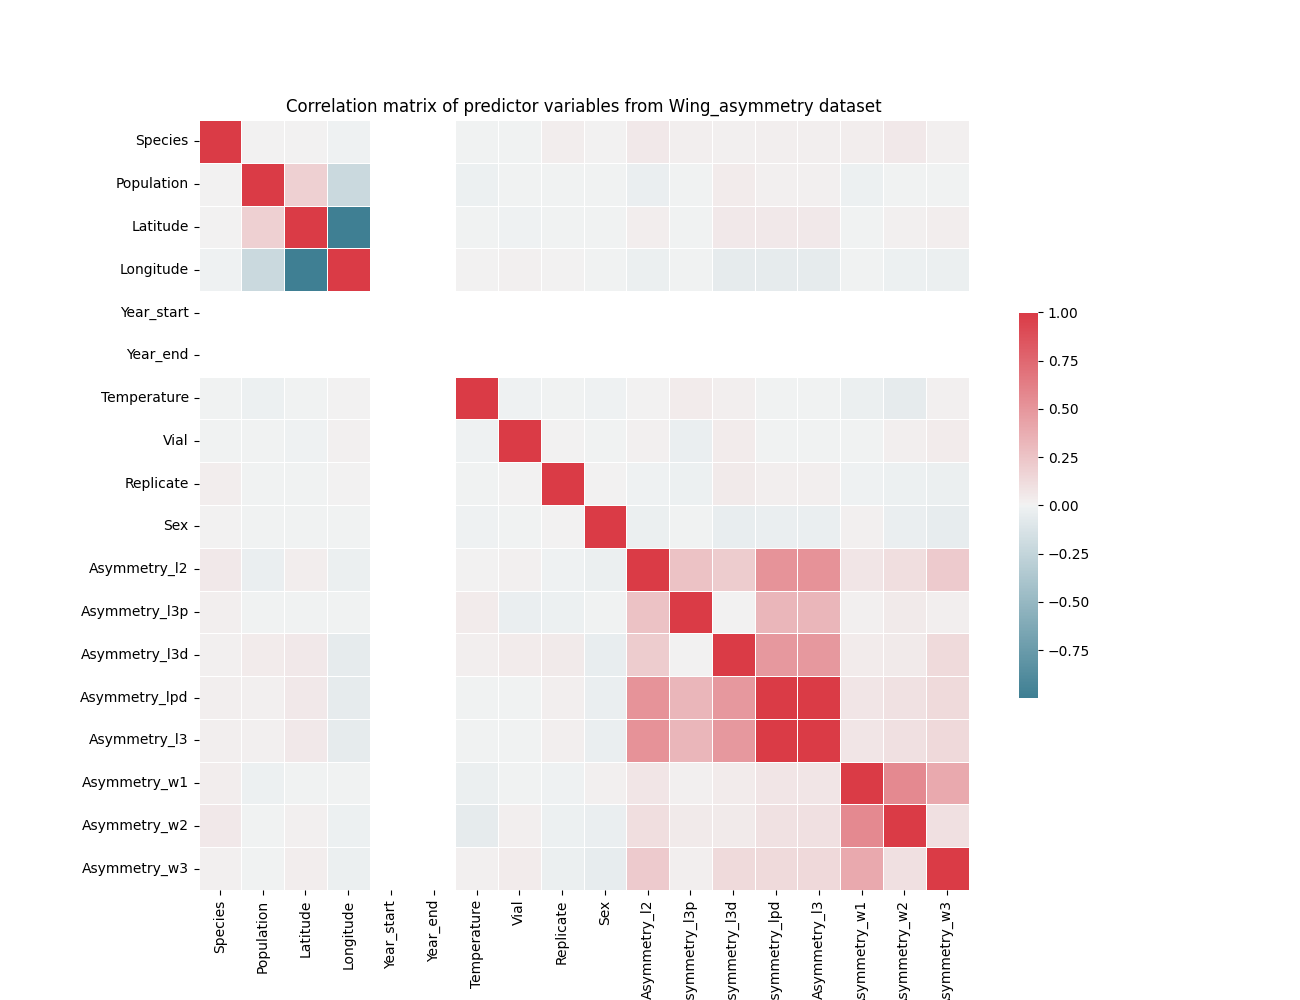
\includegraphics[width=0.8\columnwidth]{plots/Wing_asymmetry_corr_matrix.png}
    \caption{Wing Asymmetry Correlation Matrix}
    \label{fig:wing_asymmetry_corr_matrix}
\end{figure}

\newpage

The \texttt{Wing Asymmetry} dataset (which contains different asymmetry traits from the previous dataset) does show signs of correlation between wing attributes and species \& population, though this isn't as strong as the first dataset. It may, however, be a good candidate for determining temperature if that were of interest.

\begin{figure}[htb]
    \centering
    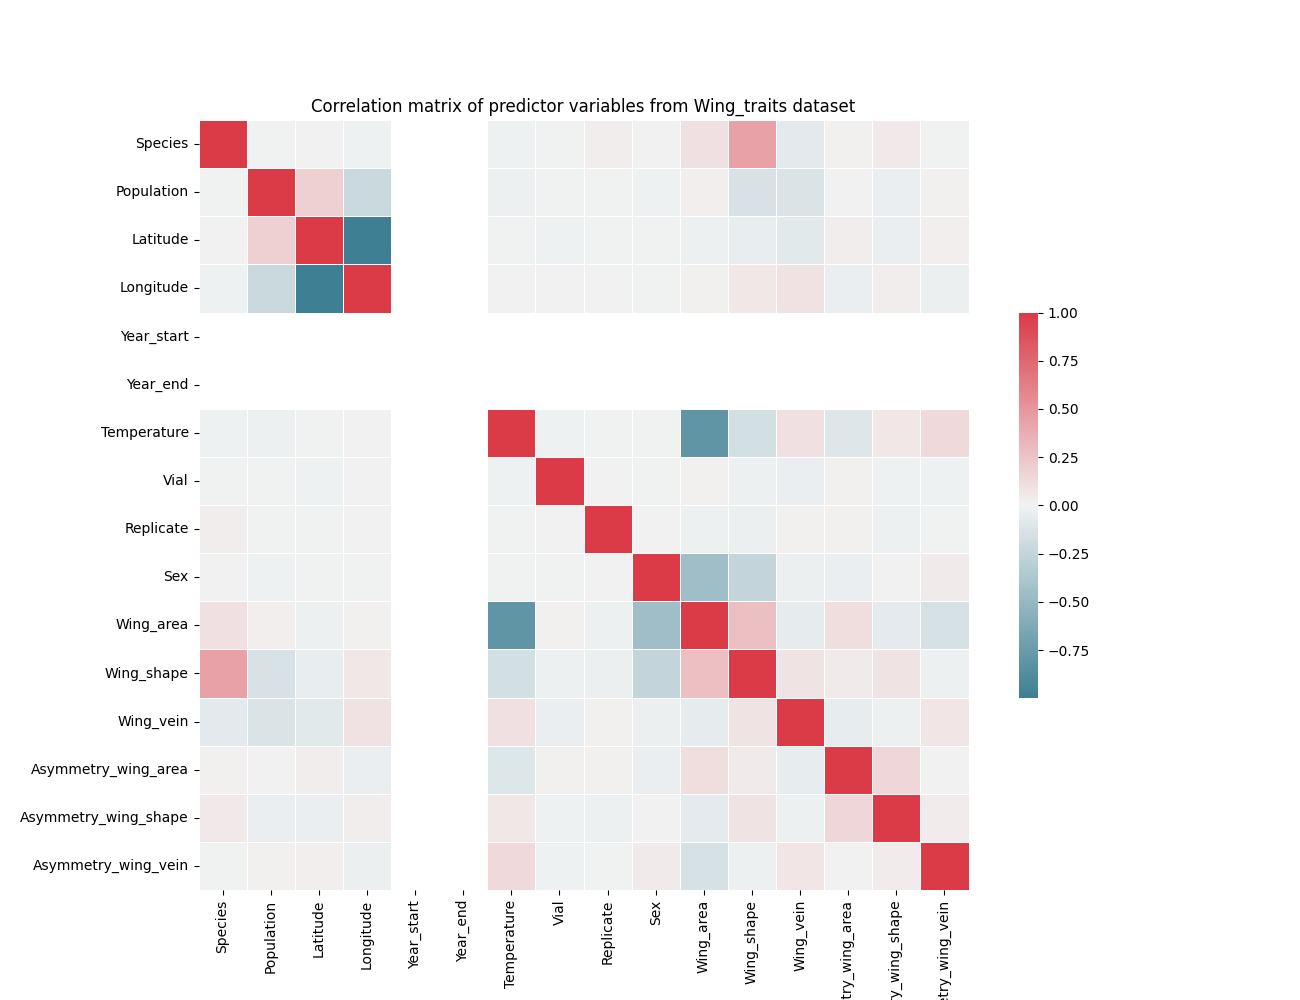
\includegraphics[width=0.8\columnwidth]{plots/Wing_traits_corr_matrix.png}
    \caption{Wing Traits Correlation Matrix}
    \label{fig:wing_traits_corr_matrix}
\end{figure}

\subsection{Objective}

While the report attached to these datasets (not this report) does provide explanation of what it is investigating, it does not provide detail on the reasoning behind doing so, other than simply to contribute to knowledge. This report will attempt to develop models which can classify both the \textbf{Species} and \textbf{Population} of fruit flies given the remaining variables collected. As per the preliminary analysis of the data, the columns \texttt{Latitude}, \texttt{Longitude}, \texttt{Year start}, and \texttt{Year end} will be removed from the dataset prior to fitting the models. \\
\\
Secondly, the report will determine a classifier which performs the best for the above object and discuss reasoning for any findings.

\newpage
\section{Hardware}

The models were trained on the following hardware

\begin{enumerate}
    \item Intel$^{\circledR}$ Core\textsuperscript{TM} i7 12700K @ 5.0 GHz
    \item 32GB DDR5 @ 5200 MT/s
    \item Samsung 990 Pro 1TB
    \item Asus ROG STRIX GeForce RTX 3080-Ti OC @ 1940 MHz with 12GB GDDR6X @ 9630 MT/s
    \item Windows 11 Pro
\end{enumerate}

CUDA compute was used to train the neural network model in a Conda environment

\bigskip
\section{Models}

The objective defined above is related to classification of the \textbf{Loeschcke} dataset, meaning only classification models will be used. In this report, the following classifiers are:
\begin{enumerate}
    \item $k$-NN
    \item Decision Tree
    \item Neural Network
\end{enumerate}

Where possible each model will be tested equally on the dataset. Note that in the case of a neural network, a single network can output multiple variables. However, this is not possible with $k$-NN or a decision tree, hence multiple classifiers will be instantiated and combined in order to make these predictions.


\newpage
\subsection{Processing of the Dataset}

In addition to filtering some of the features out, the data was pre-processed before it was fed to the models. In order of implementation, the following pre-processing steps were performed on the \texttt{Thorax and wing traits} dataset.

\subsubsection{Randomisation}

For a handful of the rows of data, some columns were missing values. Given this is fairly insignificant with respect to the $n=1731$ rows in the dataset, any decision would be acceptable here, however, in this case these values were replaced with the mean of the respective column. Replacing with the mean is a logical decision as in theory this should not have an affect the distribution of the data.

\subsubsection{Test Train Split}

For all models, a $70$ to $30$ train to test split was performed on the data. However, each model used the data slightly differently, and is further discussed below in the \textbf{Models} section of this report.

\subsubsection{Normalisation}

For both non-parametric models, the data was normalised prior to fitting the respective classifier. In the case of $k$-NN, this is an essential step to ensure the distances computed by the model use the Euclidean distance metric. Hence we want each feature to have (approximately) the same variance such that distances between variables are uniform. and decision tree models, the data was normalised, primarily because normalising does not have any affect on the model's performance. For the decision tree, this is less important, though given this is still a non-parametric learning algorithm, it remains standard practice.

\subsubsection{Encoding of non-numeric data}

For the three columns \texttt{Species}, \texttt{Population}, and \texttt{Sex}, the string values were converted into indices (e.g. $0, 1, 2, ...$) so each model could interpret them. These columns are not normalised since the values take discrete values.

\subsubsection{One hot encoding of the outputs for the neural network}

In the case of the neural network model the output variables $(y)$ were one-hot encoded. This is discussed more in detail in later sections of this report, but this was primarily done in order to enable the network to produce an output for which a loss can easily be computed. It would not make sense for discrete classes $(0, 1, 2, ...)$ to have different "losses" between them simply because the index of the class was further apart vs closer. By one-hot-encoding the output variables, each pair of classes has the same loss magnitude between them unlike numerical data where there should be a metric of loss which is proportional to the "distance" between values. \\
\\
OHE also enables multiple variables to be more easily predicted, as these can be outputted in a flattened vector far more easily by a model.

\subsubsection{PCA?}

Although PCA is discussed heavily in machine learning, it was not performed for this classification task. Primarily, there are already few features ($14$) and so further reducing the dimensionality of the data does not make sense in this case. Furthermore, a consequence of performing PCA is the loss of interpretability. For example when visualising decision boundaries, a single principal component may be comprised of many original variables meaning one cannot say for sure which of those variables contributed to the decision boundary being at a given place on the scale.


\subsection{$k$-NN}

\subsubsection{Model Setup}

As two output variables are being predicted, two separate $k$-NN classifiers were constructed, each with equal parameter setups (e.g. train set, test set, cross validation method, etc).

\subsection{Selection of $k$ - Cross Validation}

Cross validation was performed for each of the two $k$-NN classifiers (one for each output variable). A grid search over a wide range of $k$ values was performed in order to find the optimal value of $k$. To start, a $30\%$ test set was put aside and kept independent from cross validation. On the remaining $70\%$, each $k$ from $1$ through $100$ was trained on a randomly selected $\frac{4}{5}$ of the train set and validated on the remaining $\frac{1}{5}$. For each $k$, a new slicing into $5$ buckets was performed. The validation allowed us to obtain an accuracy value for each $k$ in the tested range. Once found, a final classifier was trained on a separate test set (not used in cross validation) to obtain the final results. A plot showing the accuracies for the output variable \texttt{Species} (from cross validation) of each $k$ is below:

\begin{figure}[htb]
    \centering
    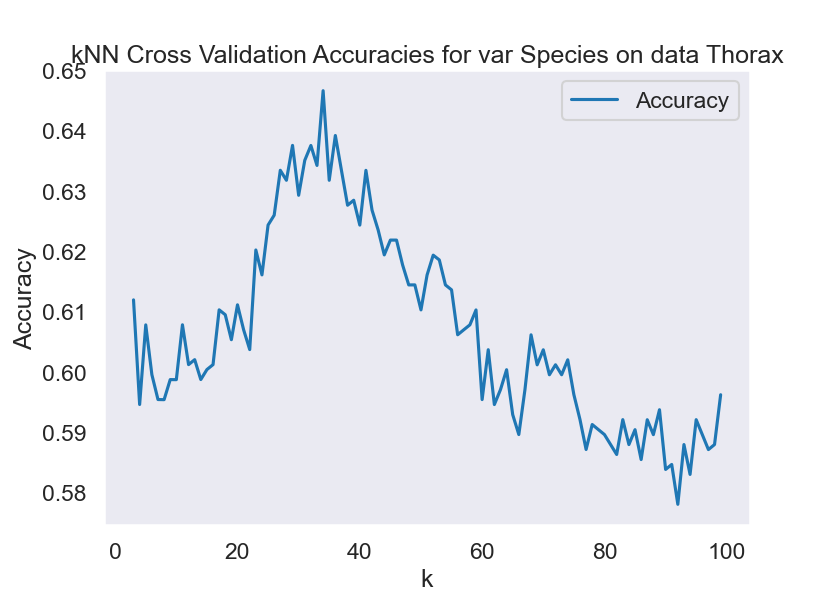
\includegraphics[width=0.8\columnwidth]{plots/Thorax_knn_accuracies_Species.png}
    \caption{$k$-NN Thorax Accuracies from Cross Validation - Species}
    \label{fig:knn_thorax_cv_accuracies_pop}
\end{figure}

The optimal value of $k$ found was $k = 34$. We observe the accuracy plot, though on a fine scale is not a smooth function. Partially this is due to the dataset being only $n = 1731$ rows which when sliced up into discrete bins used for training reduces the size of each effective training set significantly. Therefore, a small change in $k$ can result in a big change in accuracy as a result of a given train batch being "lucky" or "unlucky". Nonetheless, this does show a clear maximum on the lower end of the x-axis. \\

\newpage

A plot showing the accuracies for the output variable \texttt{Population} is shown below. Note the same range of $k$ was tested.

\begin{figure}[htb]
    \centering
    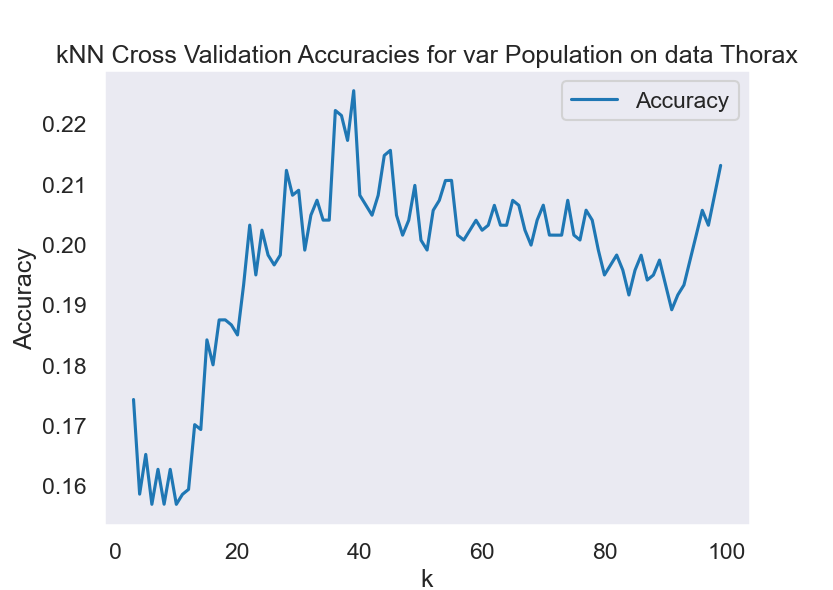
\includegraphics[width=0.8\columnwidth]{plots/Thorax_knn_accuracies_Population.png}
    \caption{$k$-NN Thorax Accuracies from Cross Validation - Population}
    \label{fig:knn_thorax_cv_accuracies_pop}
\end{figure}

We see from this graph that the optimal value of $k$ was slightly higher at $k = 39$. Both these values of $k$ are quite high which indicates there is likely significant overlap of the data. In other words, the model performs better when it can "see" points further away from the test point rather than a smaller neighbourhood.

\newpage
\subsection{Decision Tree}

The decision tree model had a similar setup to $k$-NN, however without cross validation being used. Again, two decision tree classifiers were trained since there were two output variables. Due to the small number of features ($14$), the only hyperparameter of the max tree height was chosen at $h_{\text{max}} = 10$. \\
\\
However, the decision tree was utilised for determining the importance of variables or predictors in the dataset. This was done independently for each of the two output variables. When training a decision tree, a ranking of the variables is naturally provided by the \texttt{sklearn} library. The importance of a feature is calculated based on the total reduction of the criterion (e.g., Gini impurity) brought by that feature. For each feature, \texttt{scikit-learn} under the hood sums up the reduction in impurity for all the nodes where the feature is used to split the data. These feature scores are then normalised providing a vector of relative feature importances as an output. \\
\\
There are other methods of determining variable importance, including for example Generalised Cross Validation (GCV) which essentially computes the reduction in the GCV metric as each variables is added into the classifier. The value of GCV is derived from leave-one-out cross validation (LOOCV) error and can be calculated with the following formula. It's value can be compared as features are removed (or added) to the model in order to obtain a relative ranking between them.

$$GCV(\theta) = \frac{1}{N}\sum_{i=1}^{N}\left(\frac{y_i - \hat{f}_\theta^{(-i)}(x_i)}{1-\hat{h}_i}\right)^2$$

Where:

\begin{itemize}
    \item $GCV(\theta)$ is the GCV score for a given hyper-parameter value. 
    \item $N$ is the number of data points in the dataset
    \item $y_i$ is the observed or true target value (class) for the $i$-th data point.
    \item $\hat{f}_\theta^{(-i)}$ is the model's prediction for the $i$-th data point when that data point is omitted (i.e. LOOCV)
    \item $\hat{h}_i$ is a measure of influence of the $i$-th data point in the model. For example it could be distance from the mean for each variable 
\end{itemize}

... however, this is fairly complex to implement and there isn't an existing function within a (common) library such as \texttt{sklearn} or \texttt{scikit-learn} like there exists in R under the \texttt{caret} package. \\
\\
Hence when training both the $k$-NN and neural network models, the decision tree was trained on the same data first, not for it's performance, but instead to obtain a ranking of predictor variables. This was then used in order to determine which decision boundary plots to show, given that plotting all of them would be infeasible and difficult to understand. Note the ranking of predictor variables is independent between the two output variables.

\newpage
\subsection{Neural Network}

A neural network model has the ablity to output multiple variables simultaneously. As multiple variables were being classified in this report, the neural network model did have an advantage here, though the implementation complexity is significantly higher. 

In order to output multiple class variables, $y$ was flattened into $\left[\text{data rows}, \text{output var}, \text{one-hot-encoded value}\right]$. Note that in numpy arrays / torch tensors, lengths within an axis must remain constant, so the where species has only two outputs, population has five. A workaround is to pad the one-hot-encodings to be the same length between variables. 

Computing the loss then becomes trivial since this is just a difference of two one-hot-encoded vectors - one the true $y$ and the other then predictions (either for training, validation or test). However, in order to compute accuracy, the original $y$'s (not one-hot-encoded) needed to be recovered. This also enables visualisation of the model in a decision boundary plot shown in a later section of this report. \\
\\
The model was saved meaning it could be loaded at a later stage without retraining in order to make predictions. \\
\\
The following hyperparameters were used
\begin{itemize}
    \item epochs $= 8 \cdot 10^4$
    \item batch size $= 1000$
    \item learning rate $= 2 \cdot 10^{-4}$
    \item weight decay $= 0.01$.
\end{itemize}

The number of epochs and learning rate was chosen as this achieved a good looking accuracy curve function which converged, and remained converged during the first quarter of epochs for the duration of training. The batch size is chosen arbitrarily here and more comes down to resource capacity than anything else. The Adam optimiser was used, along with Cross Entropy for the loss function. \\
\\
Note the weight decay value is the $\lambda$ which controls how much $L2$ penalty the optimiser has. A very low value was chosen here because we are already very limited for the number of features $14$ inputted into the model. Even a simple neural network model like the one used in this report should be able to fit a polynomial function with $14$ inputs, therefore, it does not make sense to penalise coefficients here.

\newpage
\section{Results}

During training of each classifier a total of $14$ predictor variables were fed as inputs for training. While this is by no means a high number of input variables, it would be impractical to plot every pairwise combination of the features as a decision boundary as there would simply be too many plots to show and analyse. We note that decision boundary plots can only really be shown in 2 dimensions (at least for now or without AR!). Instead, using the technique described in the following section, only the top $\delta = 4$ variables were considered for their decision boundary. We are interested in the top ranking predictor variables because they are the ones most likely to show a manifold like structure of the data. \\
\\
When plotting pairs of variables, the remaining features are held constant at their respective mean. This does have limitations in that some plots may misrepresent the boundaries, particularly if the size of each class isn't equal, however, it allows us to visualise the model in an easy to understand way. \\
\\
I would argue holding the non-plotted variables at their mean is superior to ploting e.g. PCA because the former method does not cause loss of interpretability of the data. From the plots below we can clearly see the regions of the classes learned by the model with respect to specific variables. Using a dimensionality reduction technique does not make sense here given the already small number of features. In the case of hundreds or thousands of input variables where many of them turn to be important, then PCA could be considered useful, however, it was not used in this report for the reasons specified above. \\
\\
In the below section, the performance of the final classifiers for both output variables is discussed, along with the the corresponding decision boundary plots according to the methodology derived above.

\subsection{Species}

Firstly, we will consider only the decision boundaries of the \texttt{Species} output variable. The top predictor variables derived from the decision tree are ranked below


\begin{itemize}
    \item \texttt{w1}
    \item \texttt{w2}
    \item \texttt{Thorax length}
    \item \texttt{wing loading}
    \item \texttt{w3}
    \item \texttt{Vial}
    \item \texttt{Replicate}
    \item \texttt{Sex}
    \item \texttt{Temperature}
\end{itemize}


In the below discussion of the each model, the decision boundary plots show the top $4$ of these features plotted pairwise, with the plotted points being the test set where the colour represents their prediction and the background representing the model's prediction across the meshgrid of the plot. Note the colours do not represent true class of the test points.

\newpage
\subsubsection{$k$-NN}

The decision boundary plot of the final $k$-NN classifier on the \texttt{Species} variable with $k = 34$ is shown below.

\begin{figure}[htb]
    \centering
    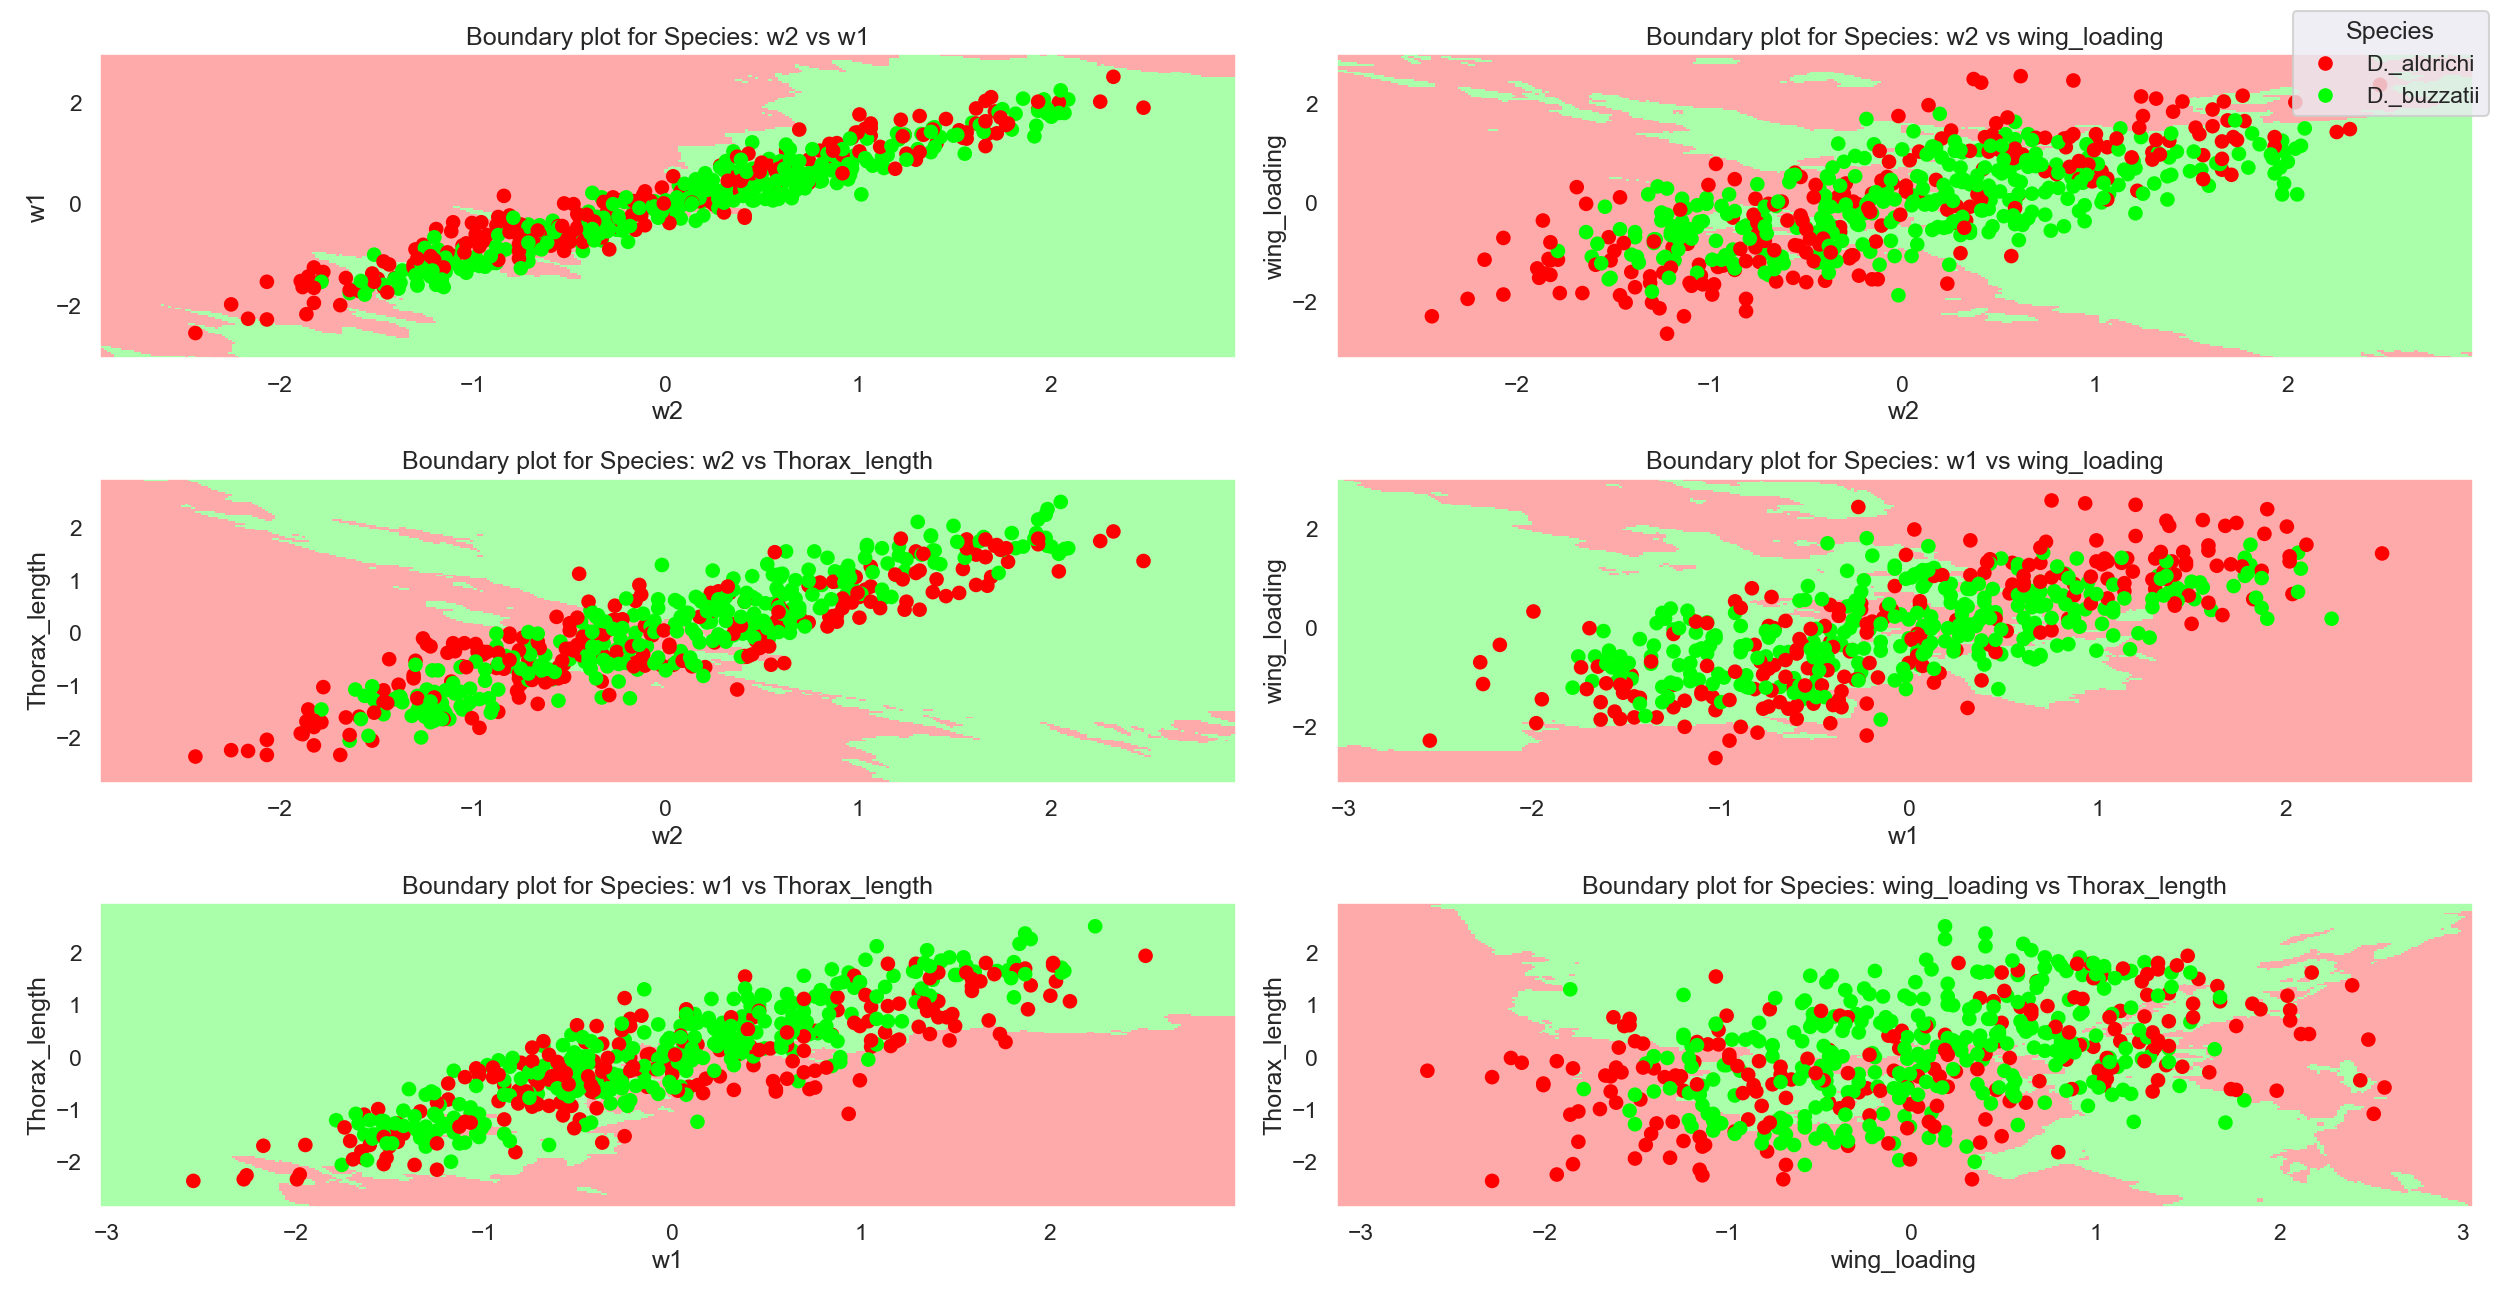
\includegraphics[width=0.8\columnwidth]{plots/knn_Thorax_decision_boundaries_Species.png}
    \caption{$k$-NN Thorax Decision Boundary - Species}
    \label{fig:knnt_thorax_db_species}
\end{figure}

The $k$-NN classifier achieved a training accuracy of $70.0\%$ and a test accuracy of $61.3\%$. It is very evident from the decision boundary plots above that the data is significantly overlapped with no clear clustering. In the bottom-right plot of \texttt{Thorax length} against \texttt{wing loading} is is clear the \texttt{D. buzzatti} (green) species appears more concentrated with respect to \texttt{wing loading} than \texttt{D. aldrichi} (red). 

It can also be seen in the \texttt{wing loading} vs \texttt{w1} plot that there is a higher concentration of \texttt{D. aldrichi} samples at the higher end of \texttt{w1} and \texttt{wing loading} than \texttt{D. buzzatti}. Although on the lower end of the scales, there isn't a clear unique cluster. 

The remaining plots do attempt to draw a boundary, though this is approximately drawn half way, or at the mean of the entire set. \\
\\
The high value of $k$ does keep very small regions in the background of the plots to a minimum however In other words, the high value of $k$ in a way prevents or at least limits overfitting of the model even in such a clustered setting. Furthermore, the generalisation gap of only of only $7.8\%$ between train and test sets further indicate the model is not overfitting to the true distribution of the data.
\newpage
\subsubsection{Decision Tree}


\begin{figure}[htb]
    \centering
    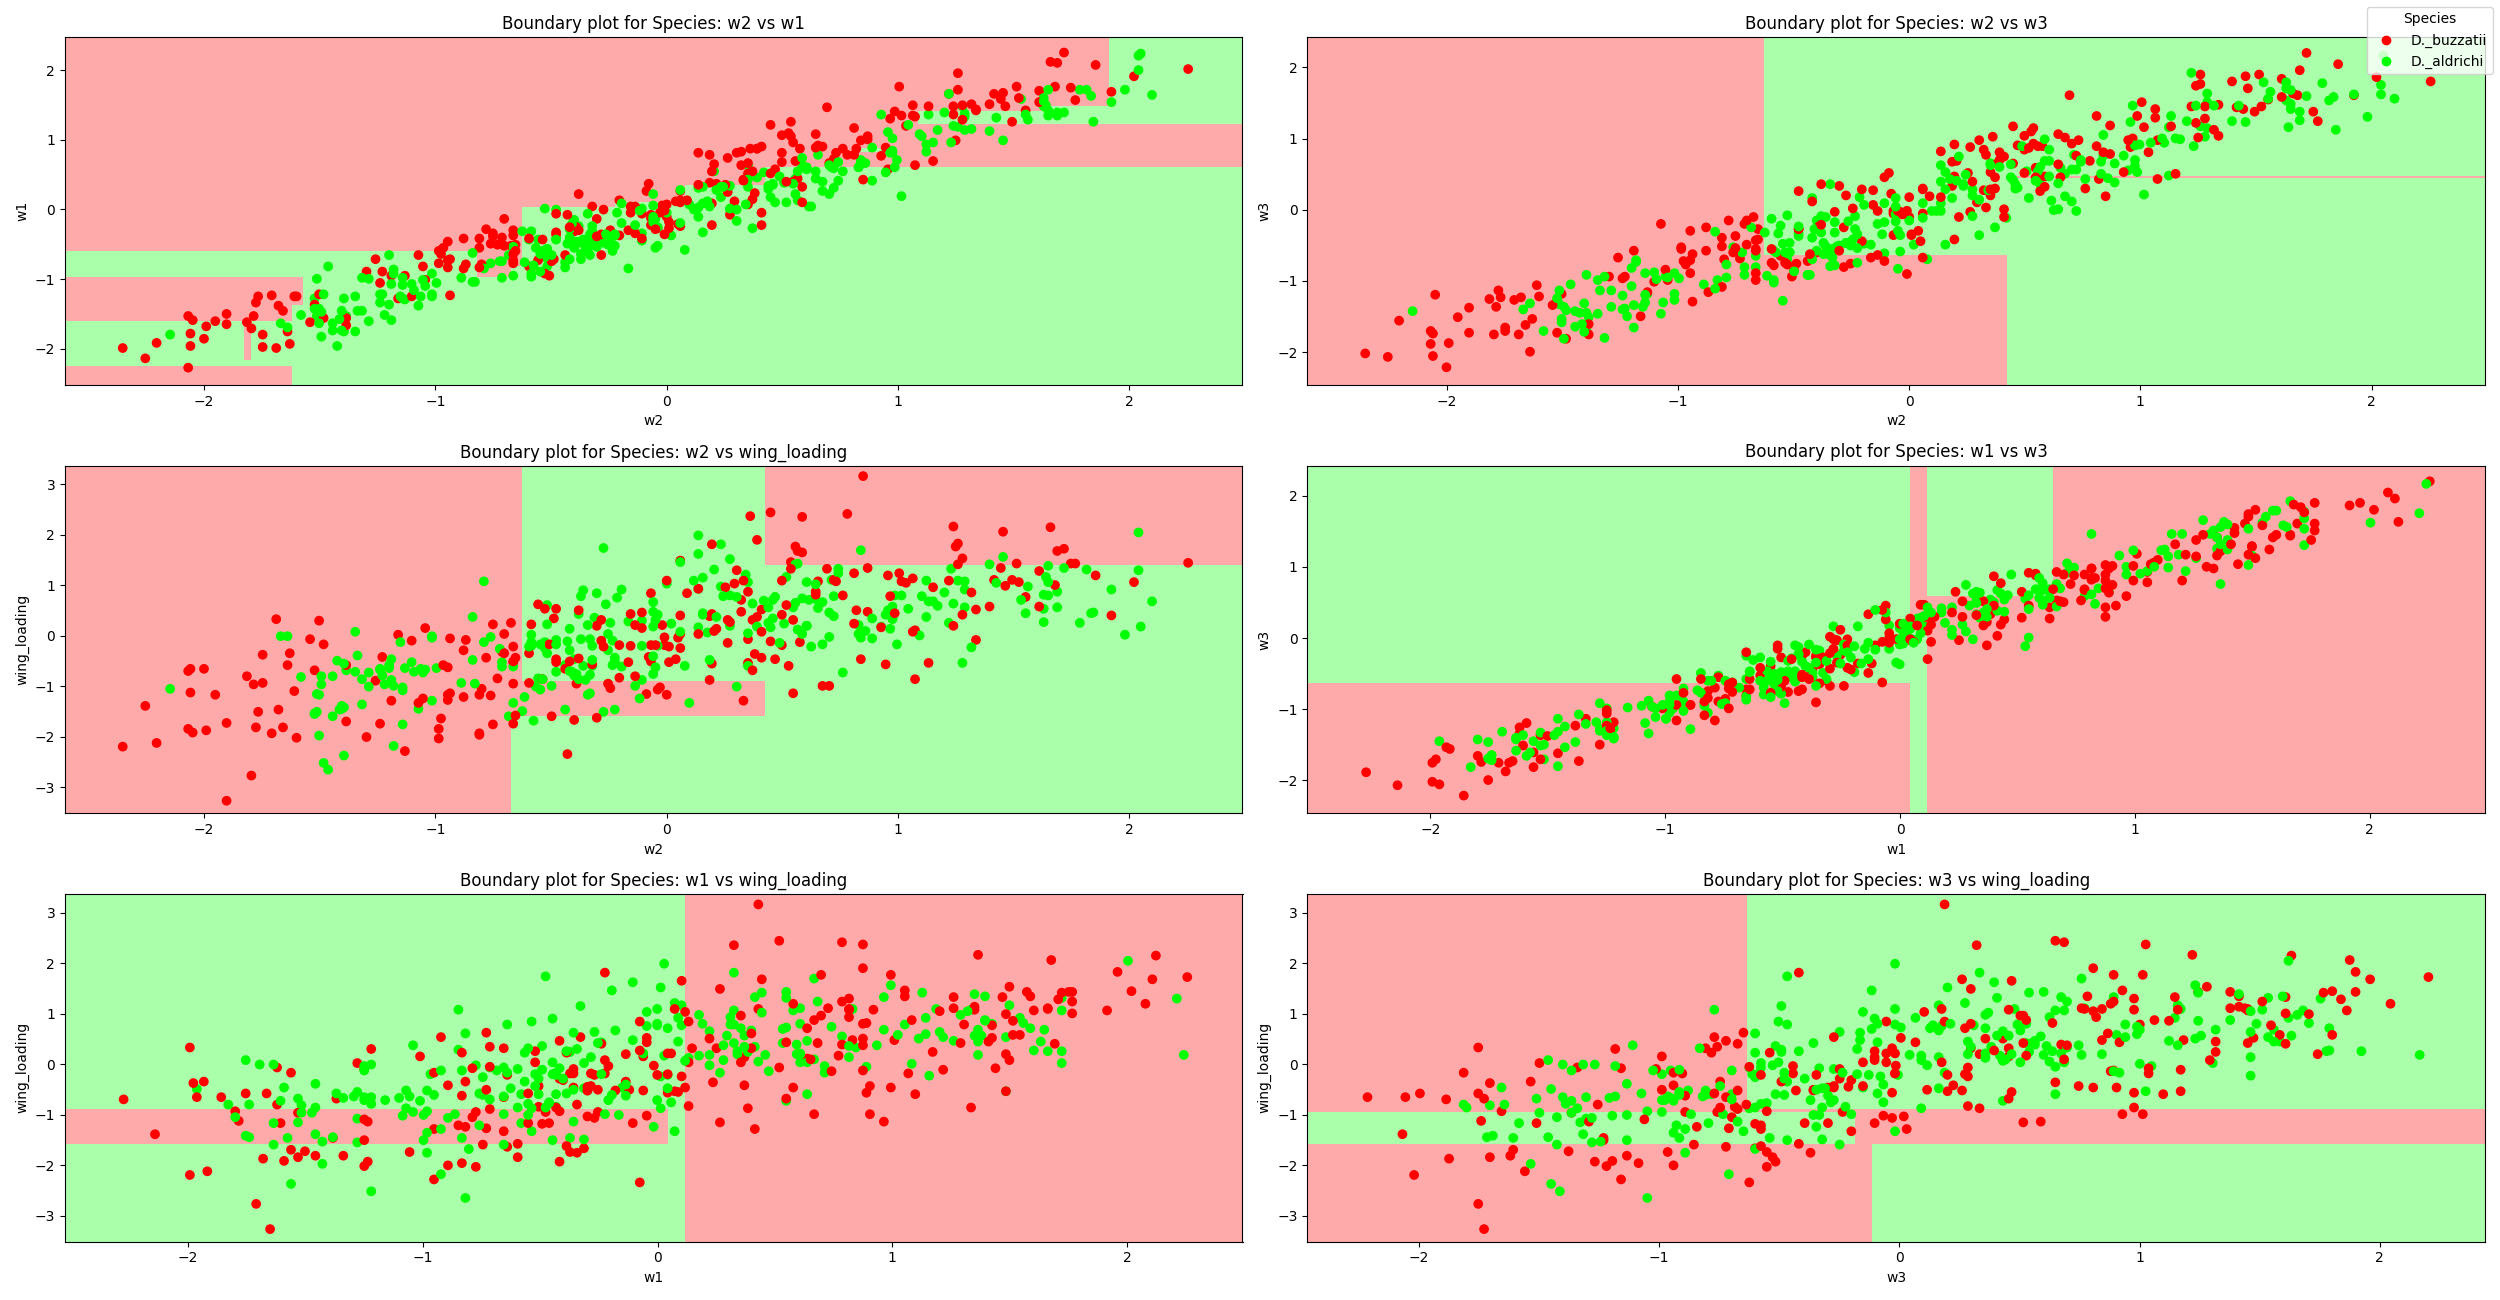
\includegraphics[width=0.8\columnwidth]{plots/dt_Thorax_decision_boundaries_Species.png}
    \caption{Decision Tree Thorax Decision Boundary - Species}
    \label{fig:dt_thorax_db_species}
\end{figure}

Interestingly the decision tree classifier performed very well achiving $83.3\%$ train and $77.1\%$ test accuracy when classifying \texttt{Species}. This very high accuracy value is not immmediatley explained by the plots above, however, due to the nature of the decision tree, it's length can be quite long, and in a 2D plot, we can effectively only visualise two layers of the tree at once, given that all other variables are fixed at their mean. \\
\\
There is, some evidence that \texttt{D. buzzatti} (red) takes higher values of \texttt{w1} than \texttt{D. aldrichi} with respect to \texttt{w2} as seen in the top-left plot, though this trend is very loose. Additionally, in the plots involving \texttt{w2}, namely the middle left and top-right, it is somewhat evident that \texttt{D. buzzatti} is more clustered on the lower end than \texttt{D. aldrichi}. \\
\\
Finally, in the bottom-left plot it is also somewhat evident that \texttt{D. aldrichi} has a visually smaller variance with respect to \texttt{Wing Loading} (y) compared with \texttt{D. buzzatti} (red). However, the model did not apply a boundary here - perhaps a deeper tree is required. \\
\\
Overall though, there are very few trends here which makes it surprising that the decision tree model was able to achieve $77.1\%$ test accuracy.

\newpage
\subsubsection{Neural Network}

\begin{figure}[htb]
    \centering
    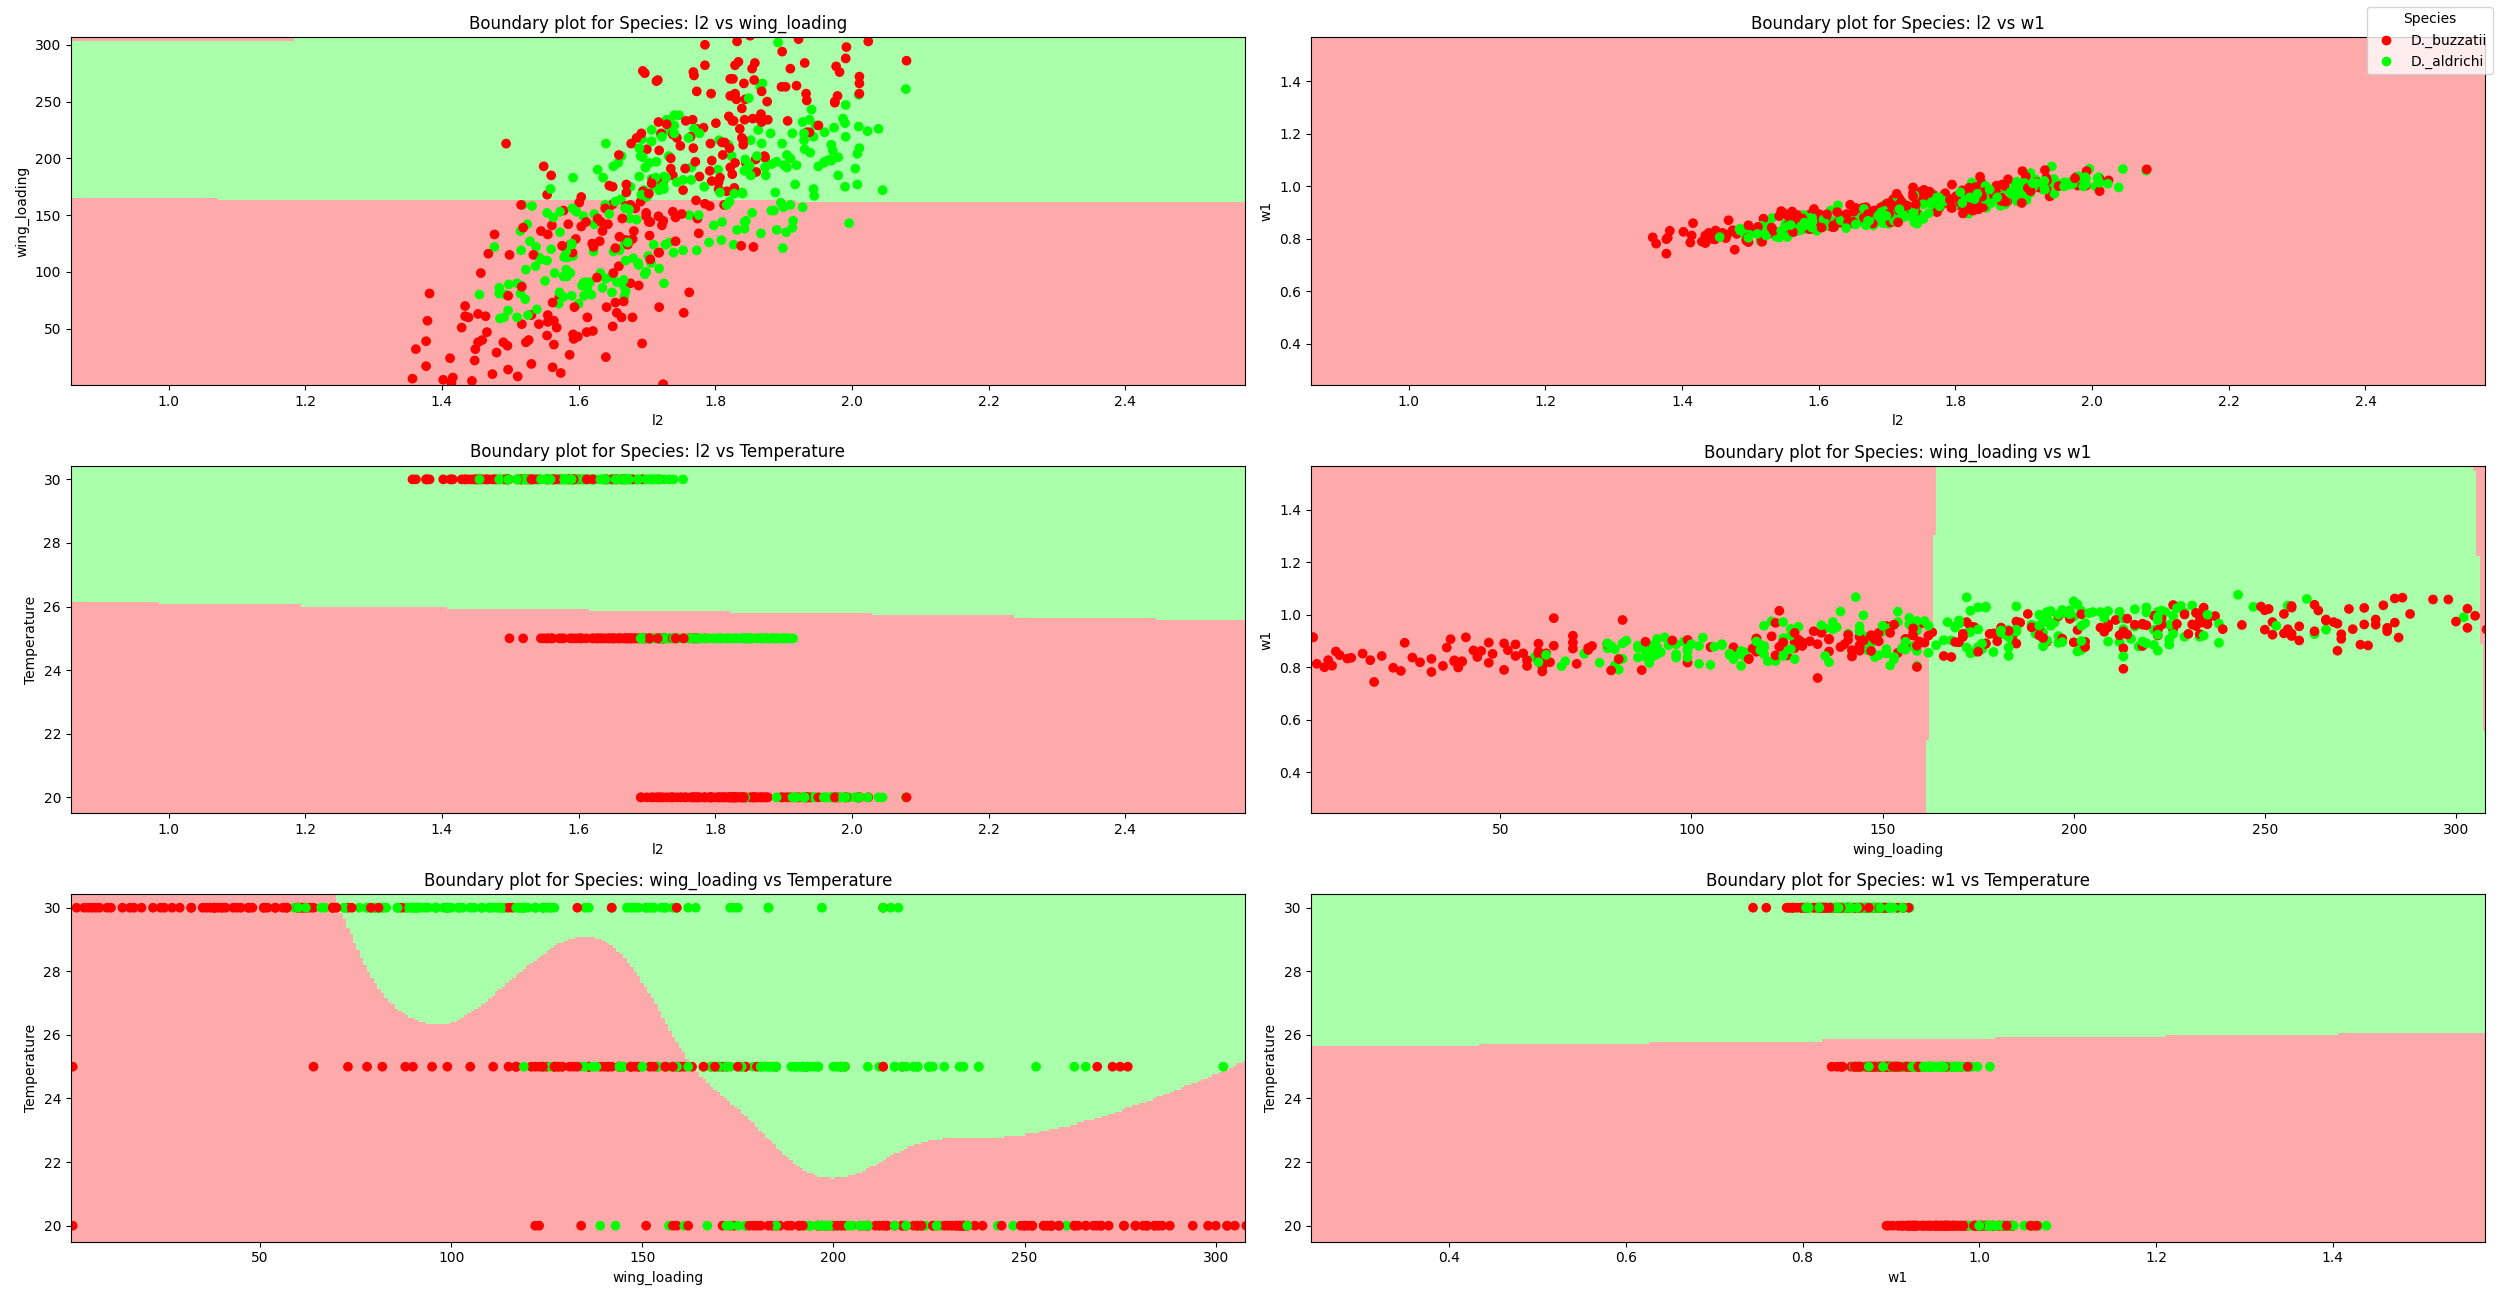
\includegraphics[width=0.8\columnwidth]{plots/nn_Thorax_decision_boundaries_Species.png}
    \caption{Neural Network Thorax Decision Boundary - Species}
    \label{fig:nn_thorax_db_species}
\end{figure}

As expected for a parametric model, the neural network learned a far smoother function than the non-parametric counterparts. This is indicated by the continuous decision boundary in the bottom-right plot (\texttt{Temperature} vs \texttt{wing loading}). Looking at the overlayed test points, this boundary appears to be the only one showing a clear difference between the two species. On the left we see more \texttt{D. buzzatti} and on the right we see more \texttt{D. aldrichi}. \\
\\
Contrast this with the plots involving \texttt{l2} and \texttt{w2} where it appears \texttt{D. aldrichi} is contained within \texttt{D. buzzatti} having the same or similar mean but a smaller variance. Unlike the decision tree model, the neural network is limited to a the constraints of a parametric function as a decision boundary. This does appear to hurt performance of the model with the NN achieving a train accuracy (averaged over the final $20,000$ epochs) of $44.4\%$ and a test accuracy of $42.6\%$. A plot showing the train and validation accuracies during training is show below.

\begin{figure}[htb]
    \centering
    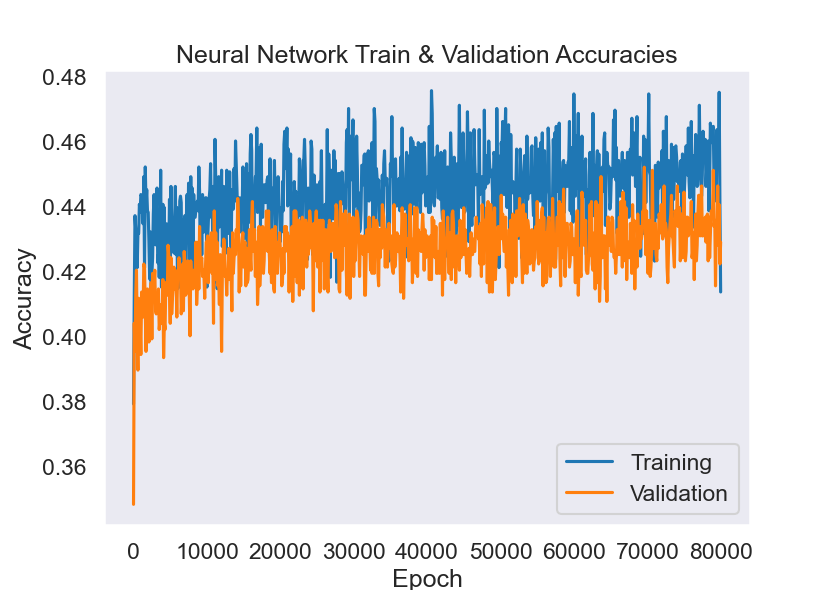
\includegraphics[width=0.6\columnwidth]{plots/nn_train_val_accuracies.png}
    \caption{Neural Network Train and Validation Accuracies}
    \label{fig:nn_train_val_acc}
\end{figure}

\newpage
While this accuracy is quite low, it is evident from the decision boundary plots above that the two species do not show a clear difference in any of the features other than perhaps \texttt{wing loading} and \texttt{temperature}. This explains the poor accuracy, though it is good to see here that the generalisation gap between train and test is quite small, indicating the model has not over fitted to the train data. \\
\\
As discussed in the data pre-processing section, if \texttt{Longitude} and \texttt{Lattitude} were included in the features, $X$, the model achieved over $90\%$ train and $85\%$ test accuracy, which corroborates the finding that these features were fixed for each class within the \texttt{Population}.

\newpage
\subsection{Population}

Secondly, we will consider only the decision boundaries of the \texttt{Population} output variable for each classifier. The top predictor variables derived from the decision tree are ranked below

\begin{itemize}
    \item \texttt{w1}
    \item \texttt{wing loading}
    \item \texttt{w2}
    \item \texttt{Thorax length}
    \item \texttt{w3}
    \item \texttt{Vial}
    \item \texttt{Sex}
    \item \texttt{Replicate}
    \item \texttt{Temperature}
\end{itemize}


\subsubsection{$k$-NN}

The decision boundary plot of the final $k$-NN classifier on the \texttt{Population} variable with $k = 39$ is shown below.

\begin{figure}[htb]
    \centering
    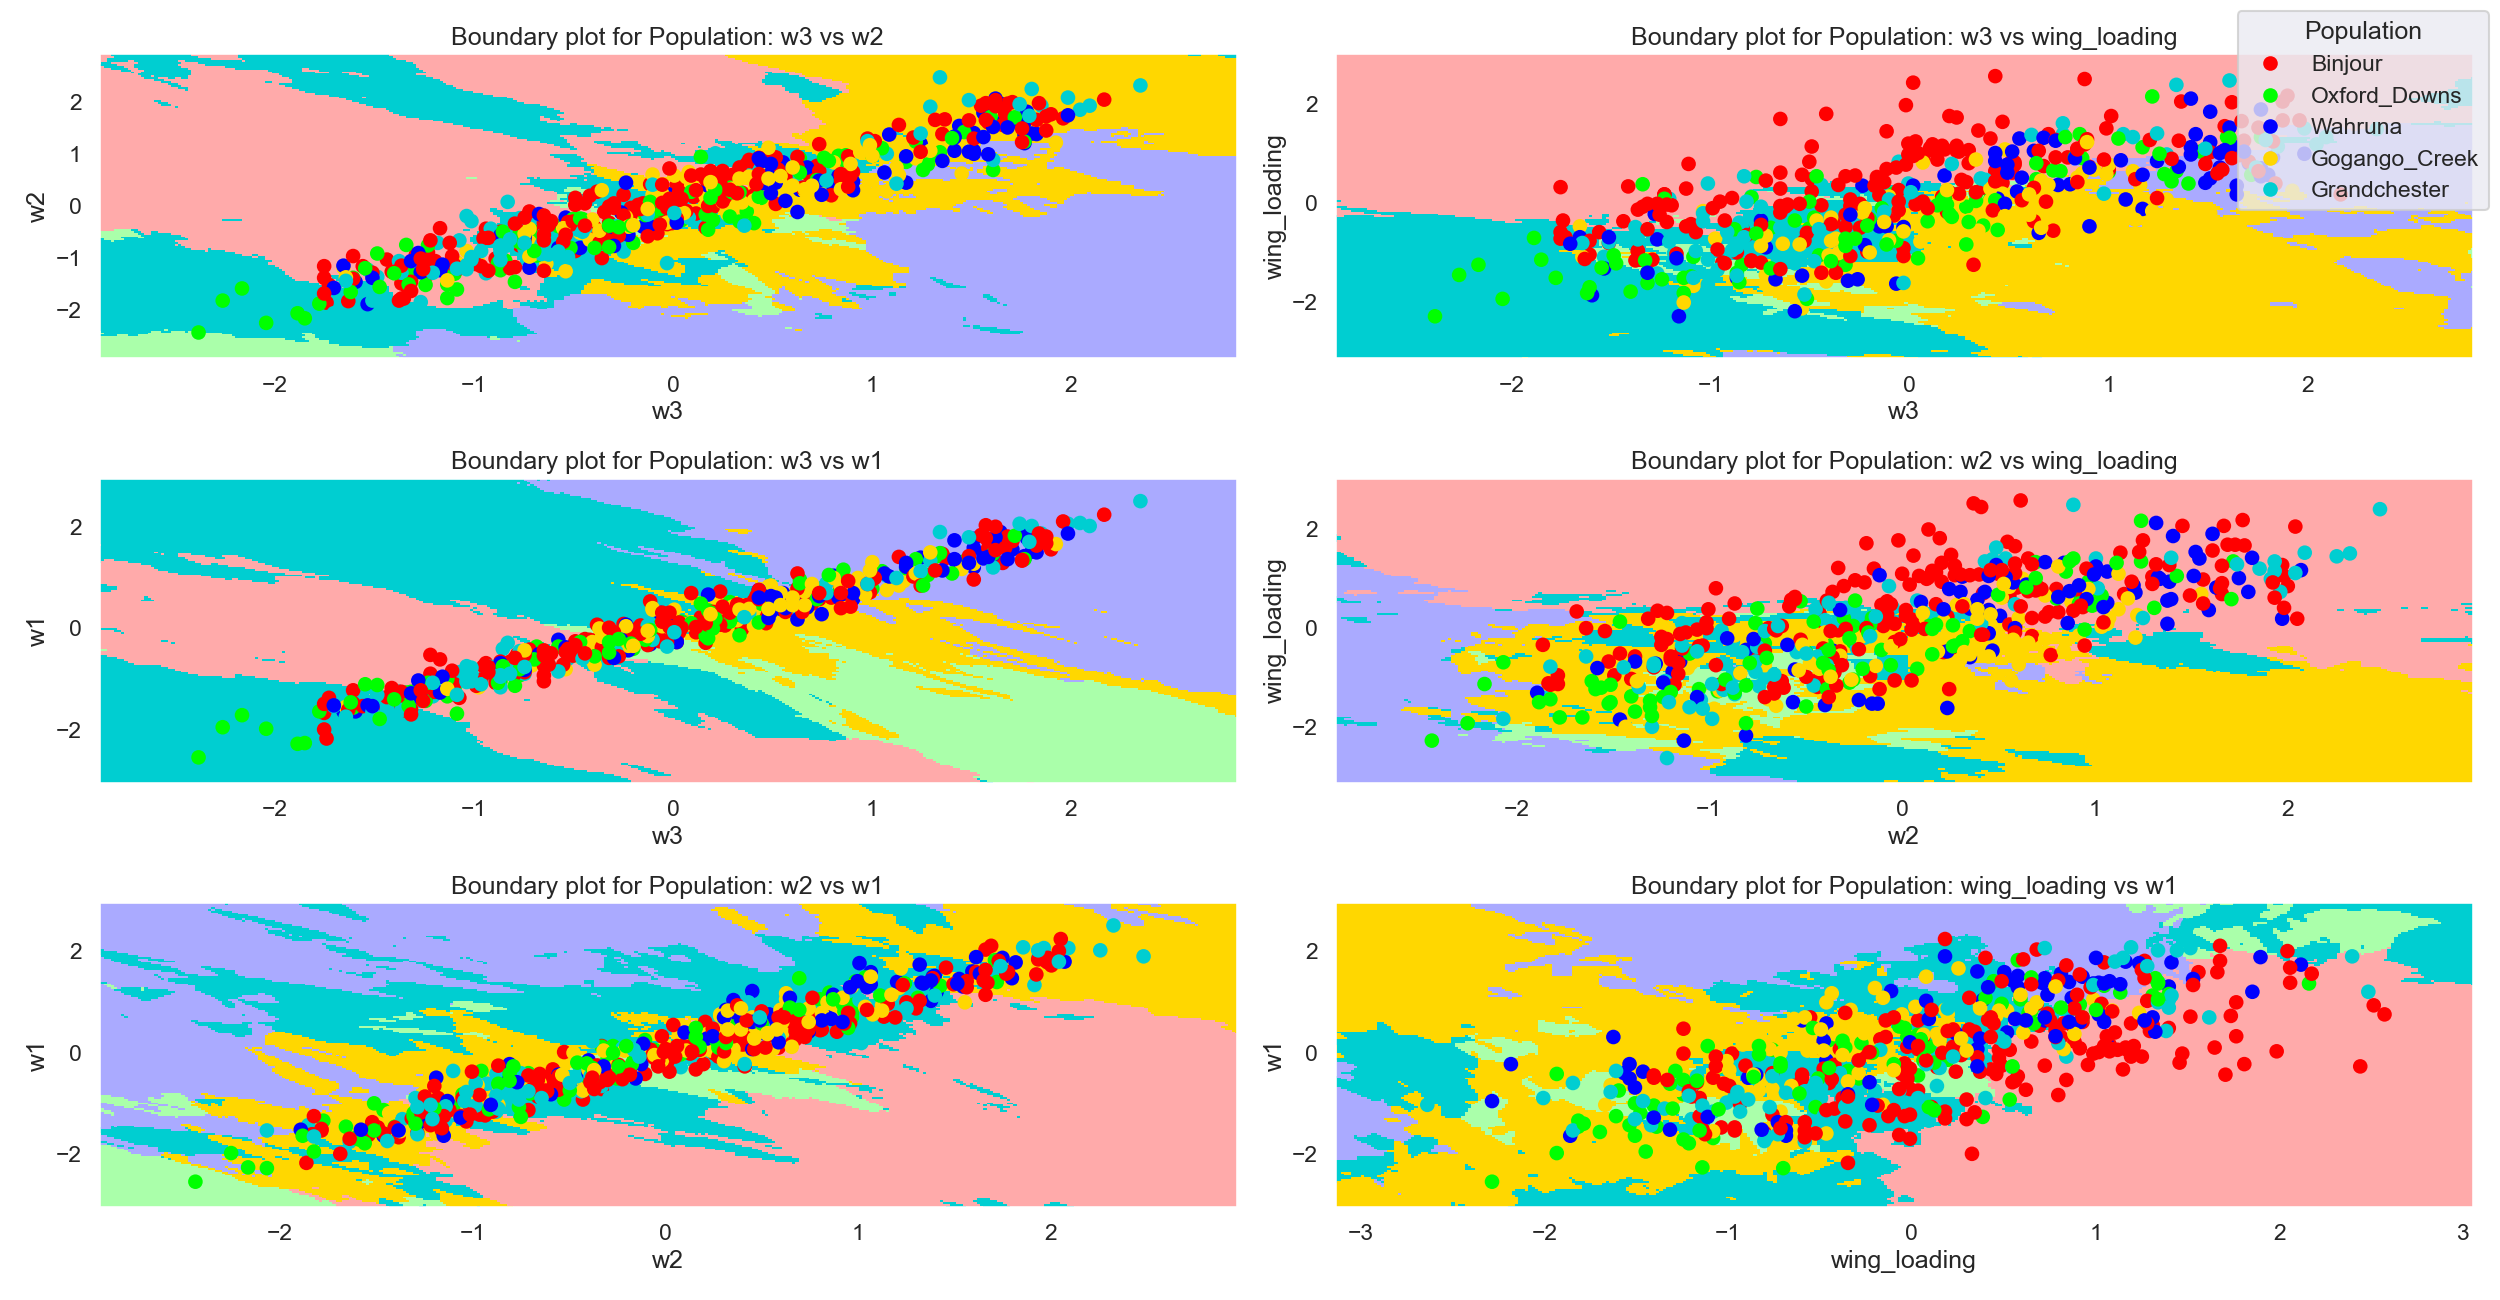
\includegraphics[width=0.8\columnwidth]{plots/knn_Thorax_decision_boundaries_Population.png}
    \caption{$k$-NN Thorax Decision Boundary - Population}
    \label{fig:knn_thorax_db_pop}
\end{figure}


From the array of decision boundary plots above, it is evident the final $k$-NN model for predicting \texttt{Population} saw a similar output compared with the \texttt{Species} final $k$-NN mode. We see again that \texttt{Thorax Length} and \texttt{wing loading} were the two best predictors as evident by the fact the decision regions have boundaries only with respect to these features. However, there are many more populations (5) than species (2), and hence the plot appears far more complex. \\
\\
The final model achieved a train accuracy of $30.6\%$ and a test accuracy of $18.9\%$. This is much lower than the \texttt{Species} $k$-NN classifier, which can partially be explained by the fact that there are simply more classes a given test point could be. Choosing randomly a classifier has a $50\%$ chance of a correct answer for the \texttt{Species} prediction, which drops to just $20\%$ when predicting \texttt{Population}. Hence one should be careful when comparing these figures. \\

\newpage
Although the plots, namely of \texttt{wing loading} vs \texttt{w1} and \texttt{wing loading} vs \texttt{w2} may appear interesting at first, given the low accuracy, it can be concluded the model did not actually perform well at distinguishing between different populations, primarily due to too much overlap of the classes. We do see different regions of classes within the plot, and these are for the most part uniquely separated, however, these could perhaps be due to slightly higher clusters of a class that simply happen to be present in that area of the hyperspace compared with the other classes. So while a high value of $k$ does limit overfitting, it may also hide the fact the model isn't understanding the distribution of the data.

\newpage
\subsubsection{Decision Tree}

\begin{figure}[htb]
    \centering
    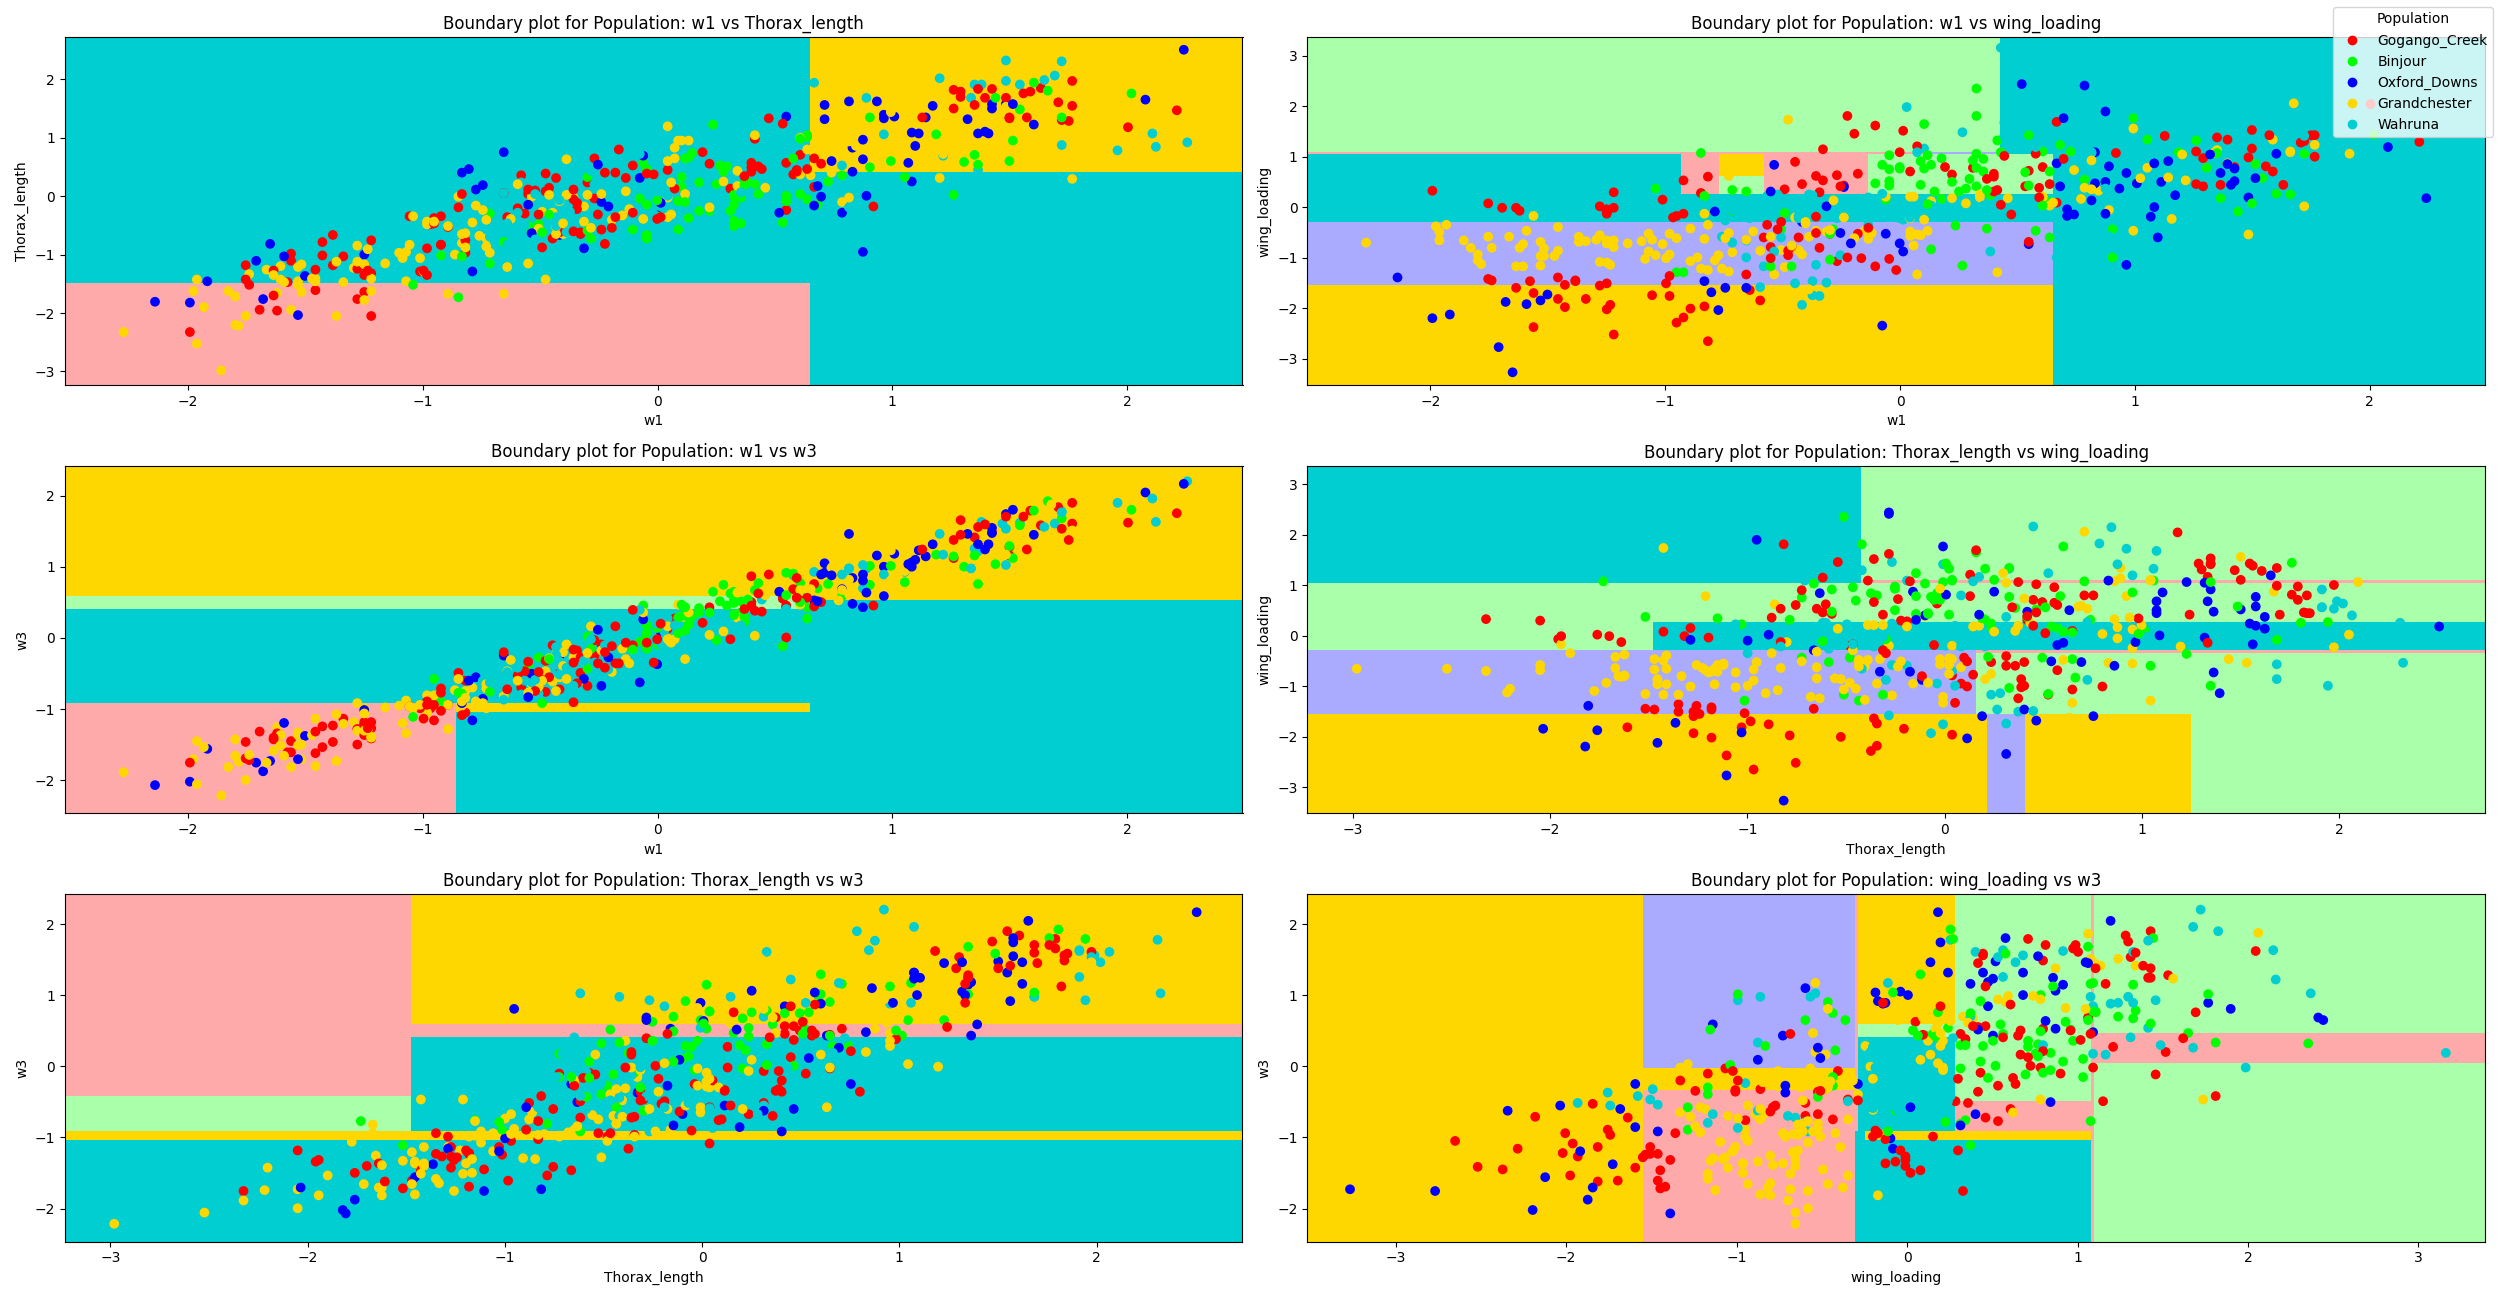
\includegraphics[width=0.8\columnwidth]{plots/dt_Thorax_decision_boundaries_Population.png}
    \caption{Decision Tree Thorax Decision Boundary - Population}
    \label{fig:dt_thorax_db_pop}
\end{figure}


When trained for classifying \texttt{Population} the decision tree model did not perform nearly as well as it did with \texttt{Species}. In training it achieved $62.6\%$ accuracy and in testing, just $22.7\%$. Again, this may come down to tweaking hyperparameters, though it is clear from the above decision boundary plots that the data lacked structure for the model to train to. \\
\\
Throughout all plots, we see test points being predicted in a different class from the underlying shaded region. This further illustrates the sharp, orthogonal decision boundaries of a decision tree. Remember that all other variables are fixed at their mean, and given there are more than two "important" features, for any given decision boundary plot, the non-plotted features play just as much of a role in determining the final predicted class as the plotted features. 

This is further corroborated by the fact that the generalisation gap was so large in this case ($39.9\%$). It indicates the decision tree was able to differentiate training plots well due to a deep tree, but was not able to capture a distribution or structure in the data in order to generalise to an independent test set.

\newpage
\subsubsection{Neural Network}

\begin{figure}[htb]
    \centering
    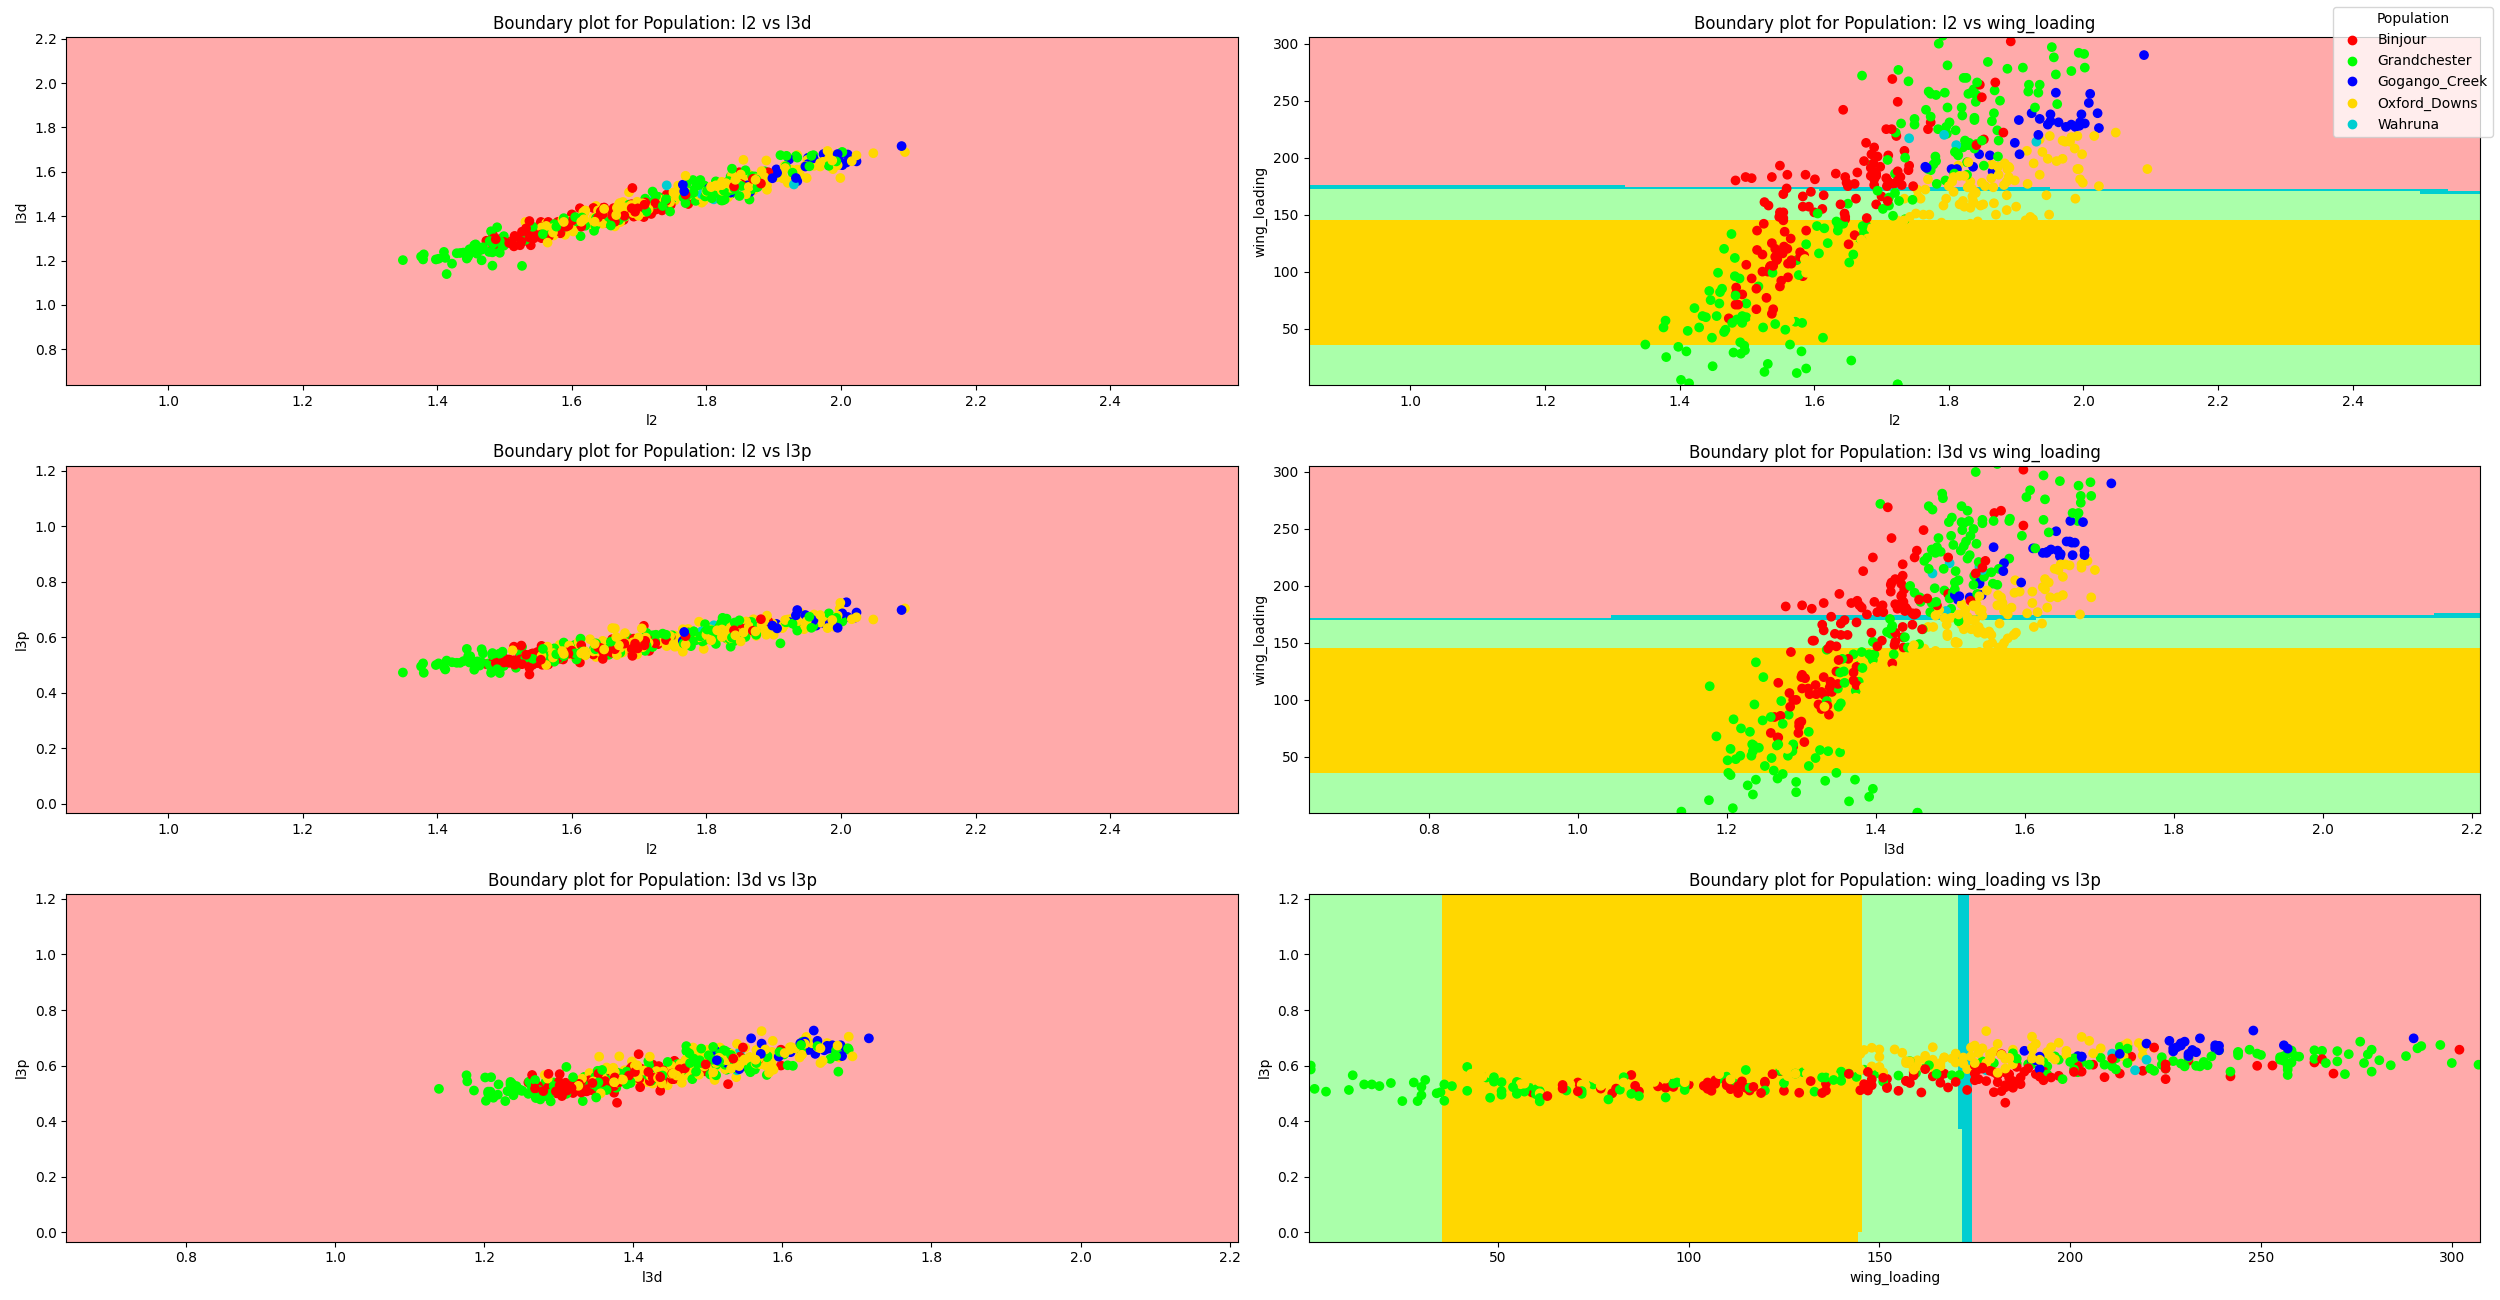
\includegraphics[width=0.8\columnwidth]{plots/nn_Thorax_decision_boundaries_Population.png}
    \caption{Neural Network Thorax Decision Boundary - Population}
    \label{fig:nn_thorax_db_pop}
\end{figure}



The neural network model also performed poorly on the Population. While the accuracy is combined with species and so we cannot tell with this data alone which output variable is most responsible, it is evident from the plots above, the high level of overlap did not allow a clear distinction between the classes. Only \texttt{wing loading} was particularly useful at separating classes


\newpage
\section{Ranking of Models}

From the results below, it might appear evident that the Decision tree model performed the best, at least for classifying species, followed closely by $k$-NN. Contrary to the numbers, given the analysis above in this report, it can be concluded both of the non-parametric models struggled to capture structure in the data. While non-parametric models are more flexible in what they can identify, they are also deceiving in that they appear to identify clusters that in reality aren't actually there. The generalisation gap for $k$-NN wasn't so bad, as a high $k$-value was used during training, but the decision tree model which lacked a grid search cross validation for its max depth suffered significantly here, especially with predicting \texttt{Population}. \\
\\
The neural network model's low accuracy is slightly deceiving as this is a combined accuracy of both \texttt{Species} and \texttt{Population}. It was noted that it did capture some structure in the data with respect to the \texttt{Temperature} in \texttt{Species} prediction, though like the non-parametric models it struggled with predicting \texttt{Population}. 

% | Model | Species Train Accuracy | Species Test Accuracy | Population Train Accuracy | Population Test Accuracy |
% |-------|------------------------|-----------------------|---------------------------|--------------------------|
% | $k$-NN            |  $70.0\%$  |       $61.3\%$        |           $30.6\%$        |         $18.9\%$         |
% | Decision Tree     |  $83.3\%$  |       $77.1\%$        |           $62.6\%$        |         $27.7\%$         |
% | Neural Network    |  $44.4\%$  |       $42.6\%$        |           $44.4\%$        |         $42.6\%$         |
\begin{table}[h!]
\centering
\begin{tabular}{|l|c:c|c:c|}
\hline
\textbf{Model} & \multicolumn{2}{c|}{\textbf{Species}} & \multicolumn{2}{c|}{\textbf{Population}} \\
\cline{2-5}
 & \textbf{Train} & \textbf{Test} & \textbf{Train} & \textbf{Test} \\
\hline
$k$-NN & 70.0\% & 61.3\% & 30.6\% & 18.9\% \\
\hline
Decision Tree & 83.3\% & 77.1\% & 62.6\% & 27.7\% \\
\hline
Neural Network & 44.4\% & 42.6\% & 44.4\% & 42.6\% \\
\hline
\end{tabular}
\caption{Model Performance on Species and Population Tasks}
\label{table:model_performance}
\end{table}


Given the results, it is quite difficult to suggest a best or worst classifier here, however, even with a lower accuracy score, it could be argued the neural network performed slightly better out of the three models. It's accuracy is a little difficult to compare, again because it is combined, but considering predicting the \texttt{Population} variable, the model outperformed simply guessing randomly, which would have resulted in a $20\%$ accuracy.


\newpage
\section{Conclusion}


In conclusion this report into classifying \texttt{Species} and \texttt{Population} from the Thorax \& wing traits dataset revealed that classifying these features is extremely difficult given the data available. It highlighted the strengths and weaknesses of three fundamentally different models. The $k$-NN and decision tree models were able to achieve fair results in this setting, however, the neural network model perhaps showed a better understanding of the underlying structure in the data.

\subsection{Improvements}

The high value of $k$ for classifying both \texttt{Species} and \texttt{Population} as selected by cross validation does make sense here, though as discussed, it does hide the fact that these supposed clusters of classes may actually not be so accurate, particularly when there are lots of classes. Hence it may be a good idea to train a final classifier also on lower values of $k$ to see the results of the decision boundary plot. \\
\\
The decision tree model did achieve a high train accuracy, however, it's test accuracy in classifying both \texttt{Species} and \texttt{Population} (notably the latter) was much lower. This indicates the model was potentially over fitted to the data. In future, performing cross validation to obtain an optimal max tree depth via a grid search may be a good step. \\
\\
Additionally, the decision tree's high performance in classifying species would benefit from further investigation, perhaps using bagging (e.g. a Random Forest) to corroborate this finding, as it does not appear clear from the visualisations presented that the model captured the underlying distribution of the species data. \\
\\
Finally, given the difficulty of this classification task, combining the other two datasets with the \texttt{Thorax and wing traits} as used would be an interesting extension to this report. It could perhaps investigate if adding additional features to the training set helps (or doesn't help) to increase performance of the different models.


\newpage
\section{References}

\begin{itemize}
    \item Australian Government Department of Agriculture, Fisheries and Forestry. (2023) 'Fruit flies in Australia', Department of Agriculture, Fisheries and Forestry. Available at: \href{https://www.agriculture.gov.au/biosecurity-trade/pests-diseases-weeds/fruit-flies-australia}{https://www.agriculture.gov.au/biosecurity-trade/pests-diseases-weeds/fruit-flies-australia} (Accessed: 02 May 2024).
    \item VarImp GitHub Source - \href{https://github.com/topepo/caret/blob/master/pkg/caret/R/varImp.R}{https://github.com/topepo/caret/blob/master/pkg/caret/R/varImp.R}
\end{itemize}



\end{document}
